\documentclass[12pt]{jarticle}
\usepackage[utf8]{inputenc}
\usepackage[top=30truemm, bottom=30truemm, left=20truemm, right=20truemm]{geometry}
\usepackage{amsmath}
\usepackage{amssymb}
\usepackage{mathtools}
\usepackage{siunitx}
\usepackage{bm}
\usepackage[dvipdfmx]{graphicx}
\usepackage[dvipdfmx]{color}
\usepackage[subrefformat=parens]{subcaption}
\usepackage{booktabs}
\usepackage{tabularx}
\usepackage{tocloft}
\usepackage{enumerate}
\usepackage{url}
\usepackage{multirow}
\usepackage{caption}
\usepackage{enumitem}
\usepackage{makecell}
\usepackage{array}

\numberwithin{equation}{section}    % 数式番号にセクション番号をつける
\numberwithin{figure}{section}      % 図番号にセクション
\numberwithin{table}{section}      % 図番号にセクション

% \renewcommand{\figurename}{Fig.}    % 図 -> Fig.
% \renewcommand{\tablename}{Table }   % 表 -> Table

\renewcommand{\baselinestretch}{1.1}

\newlength{\figcaptionskip}
\setlength{\figcaptionskip}{5pt} % 図のキャプション間隔
\newlength{\tabcaptionskip}
\setlength{\tabcaptionskip}{-5pt} % 表のキャプション間隔
\captionsetup[figure]{skip=\figcaptionskip}
\captionsetup[table]{skip=\tabcaptionskip}

\setlist[enumerate]{topsep=5pt, partopsep=5pt, itemsep=0pt, parsep=0pt}
\setlength{\topsep}{5pt}
\setlength{\partopsep}{5pt}


\begin{document}

\begin{titlepage}
    \begin{center}
        {\Large 2024年度後期 修士論文}
        \vspace{120truept}

        {\huge 深層学習による口唇音声変換に関する研究}
        \vspace{30truept}

        {\huge A Study on the Conversion from Lip-Video to Speech Using a Deep Learning Technique}
        \vspace{120truept}

        {\Large 2025年月日}
        \vspace{10truept}

        {\Large 九州大学芸術工学府音響設計コース}
        \vspace{70truept}

        {\Large 2DS23095M}
        \vspace{10truept}

        {\Large 南 汰翼}
        \vspace{10truept}

        {\Large MINAMI Taisuke}
        \vspace{30truept}

        {\Large 研究指導教員 鏑木 時彦 教授}
    \end{center}
\end{titlepage}

\section*{概要}
\thispagestyle{empty}
\clearpage

\setcounter{tocdepth}{2}
\tableofcontents
\thispagestyle{empty}
\clearpage

\pagestyle{plain}
\setcounter{page}{1}

\section{序論}
\subsection{背景}
音声は基本的なコミュニケーションの手段であり、人と人とのコミュニケーションの場面において、重要な役割を果たしている。音声は、肺からの呼気流による声帯の振動が音源波を生成し、声道特性に伴ったフィルタリングと口唇からの放射特性に従って生成される。これより、音声の生成には音源を作り出す声帯やその制御のための喉頭、舌や口唇といった調音器官の働きが重要となる。しかし、癌などの重い病気で喉頭を摘出した場合、音源波を生成することができなくなるため、これまで通り発声を行うことが不可能になってしまう。このようなコミュニケーション機能の喪失に対し、現在でも電気式人工喉頭や食道発声、シャント発声といった代用音声手法が存在する。電気式人工喉頭では、専用の発振器を顎下に当てて振動を加えることにより、それを音源とした発声を行う。発振器を用意すれば容易に発声することが可能であるが、生成される音声のピッチが発振器の振動に依存してしまうため、抑揚のない単調な音声になってしまう。食道発声では、まず口や鼻から食道内に空気を取り込み、その空気を逆流させることで食道入口部の粘膜を振動させることによって発声する。電気式人工喉頭と違って道具を必要とせず、ピッチも本人が調節できるが、その習得に長期間の訓練を要する。シャント発声では、手術によって気管と食道を繋ぐ管を設ける。これにより、息を吐き出す際に設けられた喉の穴を手で塞ぐことによって肺からの呼気流が食道に流れる。そのため、食道発声と同様に粘膜の振動を音源とし、発声することが可能となる。習得は容易であり、比較的自然に話すことが可能となるが、設けられた管を交換するための定期的な手術が必要となる。このように、現在用いられている代用音声手法にはそれぞれデメリットが存在する。

そのため、本研究ではビデオカメラで撮影した口唇の動きから音声合成を行うことによる、新たな代用音声手法を検討する。本来、音声は声帯の振動や声道の形状に依存して生成されるものであり、口唇の動きのみから音声波形を直接推定することは困難である。そこで、近年画像や自然言語処理、音声といった分野において成果を上げている深層学習を使用し、データ駆動型の方法で口唇の動きと音声の間の関係を学習することで推定を行う。これにより、従来の代用音声手法よりも自然性の高い音声を、訓練や定期的な手術の必要なく提供することを目指す。

これまでの動画音声合成は英語が中心に検討が進んでおり、近年ではYouTube上のデータを収集、処理することによって構築した大規模データセット~\cite{afouras2018lrs3,chung2018voxceleb2}を用いることで、大規模で表現力の高いモデルが構築可能となっている。これにより、従来行われてきた教師あり学習のみならず、動画と音声の関係性を自己教師あり学習(Self Supervised Learning; SSL)によって学習し、そのモデルを動画音声合成や、動画からテキストを推定するVisual Speech Recognition(VSR)にFineTuningするアプローチが提案され、その有効性が示されている。自己教師あり学習モデルにもいくつかの種類があり、近年多くの研究で応用例のあるAVHuBERT~\cite{shi2022learning}は、動画・音声の入力領域においてマスクされた区間の予測と、予測対象の更新を繰り返して学習を進めていくモデルである。予測対象の更新は5回行われ、1回目は音声波形から計算されるMFCCをクラスタリングした結果を利用するが、2回目以降はモデルの中間特徴量をクラスタリングした結果を新たな予測対象に設定する。更新のたびに再度モデルをランダム初期化して再学習するが、その予測対象の複雑さが増していくことによって学習を促進するようなメカニズムとなっている。また、これに類似したVATLM~\cite{zhu2023vatlm}は、動画と音声のみならずテキストも加えた学習によって、精度改善を達成した。その他、StudentとTeacherという二つのネットワークを利用し、Teacherから出力される特徴量をStudentがマスクされた入力から予測することによって学習を進めるRAVEn~\cite{haliassos2022jointly}やAV-data2vec~\cite{lian2023av}、RAVEnの改善版として提案されたBRAVEn~\cite{haliassos2024braven}など、多くのモデルが提案されている。

近年の動画音声合成やVSRでは、こういったSSLモデルを動画からの特徴抽出器として活用しつつ、さらなる工夫によって精度改善を達成している。動画音声合成について、~\cite{kim2023lip_multitask}では予測対象として従来用いられてきたメルスペクトログラムに加え、テキストを予測するマルチタスク学習手法を提案した。損失においては上記の二つに加え、予測したメルスペクトログラムを事前学習済みのASR(Automatic Speech Recognition)モデルに入力して得られる特徴表現も採用した。音声波形はメルスペクトログラムに対してGriffin-Limアルゴリズムを適用することで獲得しており、従来のメルスペクトログラムのみを損失とする手法に対して客観評価指標における改善を達成した。これに続き、~\cite{choi2023intelligible}では前述した手法がテキストアノテーションされたデータのみにしか用いることができないという課題を解消するため、テキストと同様に言語的な情報を持つと考えられている、音声SSLモデルのHuBERT\cite{hsu2021hubert}から得られた離散特徴量(HuBERT離散特徴量とする)を利用する手法を提案した。また、予測されたメルスペクトログラムとHuBERT離散特徴量の両方を入力とするMulti-input Vocoder、Multi-input Vocoderの学習時にメルスペクトログラムにノイズをかけるデータ拡張を合わせて提案し、客観評価と主観評価の両方で改善を達成した。加えて、ここではAVHuBERTの転移学習についても合わせて検討が行われ、これによってさらに性能を改善できることを示した。手法~\cite{choi2023intelligible}に関連して、上記のようなマルチタスク学習手法以外にも、HuBERT離散特徴量やHuBERT連続特徴量(離散化しない場合を指す)を音声波形までの中間特徴量として扱う手法は提案されている。例えば、~\cite{hsu2023revise}ではメルスペクトログラムの推定を行わず、HuBERT離散特徴量のみを推定して音声波形に変換する手法が提案された。~\cite{choi2023intelligible}では離散化におけるクラスタ数を200にしていたのに対して、~\cite{hsu2023revise}ではクラスタ数を2000と大きく取っている点で実装が異なっている。メルスペクトログラムを省略する分情報圧縮の程度を軽減することで、音声波形への変換に十分な情報を保持する目的があると考えられる。また、\cite{choi2023intelligible}や\cite{hsu2023revise}ではAVHuBERTを直接動画音声合成にFineTuningしていた一方で、~\cite{sahipjohn2023robustl2s}ではAVHuBERTをVSRによってFineTuningし、その後重みを固定した上で特徴抽出器として利用するアプローチを提案している。動画音声合成モデルは、VSRでFineTuningしたAVHuBERTから得られる動画特徴量を入力とし、HuBERT特徴量を予測するネットワークを導入して、HuBERT特徴量のみから音声波形に変換するボコーダを利用することで構築される。ここではHuBERT特徴量として連続値および離散値の両方が検討され、連続値を用いる場合の方が客観評価指標が改善することを報告している。検討された離散値のクラスタ数が100であったため、\cite{hsu2023revise}の結果と合わせると、HuBERT離散特徴量のみで音声波形に変換するアプローチを取るのであれば、クラスタ数を十分大きく取る必要があることが予想される。

一方VSRについて、~\cite{yeo2024akvsr}では音声認識を利用して言語情報を格納したメモリを用意し、メモリと動画特徴量の間でアテンションをとることによって、ネットワーク内部で言語情報との関連を考慮する構成を提案した。また、~\cite{cheng2023opensr}ではAVHuBERTが動画あるいは音声のどちらを入力とした場合でもクロスモーダルな特徴量を返すことに着目し、音声認識デコーダに組み合わせるAVHuBERTのFew-shot Learning、Zero-shot Learningによる転移学習を検討した。加えて、同様に音声認識デコーダを転移学習するアプローチであるが、事前学習済みモデルの重みを固定し、動画特徴量から音声認識モデルの中間特徴量を予測するネットワークのみを新たに学習することで、両者を合併するようなアプローチ~\cite{djilali2023lip2vec}も提案されている。さらに、静止画像と音声から動画を合成するネットワークを構築し、音声認識用のデータセットを用いてVSRの学習データを大量に合成するデータ拡張手法~\cite{liu2023synthvsr}や、事前学習済みの音声認識モデルによって教師なしデータにラベリングを行うデータ拡張手法~\cite{ma2023auto}、10万時間分の教師ありデータを新たに増強した研究~\cite{chang2024conformer}など、大規模な学習データを確保することで精度改善を達成した例も報告されている。

上記の研究は英語データを用いたものであったが、VSRにおいては英語以外の言語に焦点を当てた研究や、多言語対応モデルの構築も検討が進んでいる。~\cite{zinonos2023learning}ではRAVEnを利用し、英語に加えてスペイン語、イタリア語、ポルトガル語など計6種類の言語が含まれるデータセット~\cite{ephrat2018looking,salesky2021multilingual,zhao2019cascade}を用いて多言語モデルの構築を検討した。結果として、教師ありデータの少ない英語以外の言語に対する、多言語モデルの有効性が明らかとなった。また、~\cite{kim2023lip_vsr}では英語データで学習されたAVHuBERTを用いつつ、特定の言語ごとに構築した音声認識モデルのデコーダを転移学習することで、特定言語ごとにモデルを構築するアプローチを提案した。さらに、~\cite{yeo2023visual}では音声認識モデルであるWhisperを利用し、教師なしデータへのラベリングによるデータ拡張を行うことで、上記二つのアプローチを超える精度を達成した。

本研究では、近年の主流とも言える英語大規模データセットを用いた実験は計算機のスペックの都合上難しく、世界的に見て日本語での動画音声合成の検討例が少ないことも考慮して、文献~\cite{taguchi,esaki}で収録された日本語データを用いて研究を行うこととした。英語データと比較して小規模なデータである分性能に課題を抱えたが、予備実験として英語データで学習されたAVHuBERTのFineTuningを検討したところ、スクラッチで構築したモデルと比較して、より高い精度を示すことが明らかとなった。これは、英語データを用いた事前学習済みモデルの多言語対応を検討した先行研究の傾向にも一致する結果であり、日本語においても同様に有効なモデルだと考えられる。しかしながら、それでも依然として合成音声の品質は低く、自然音声に迫る合成音は実現されていないことが課題である。

\subsection{目的}
本研究の目的は、動画音声合成によって得られる合成音声の品質を向上させることである。近年高い精度を達成した手法~\cite{choi2023intelligible}では、AVHuBERTの利用および、メルスペクトログラムと音声SSL離散特徴量を利用したマルチタスク学習が採用されている。その他にも近年高い精度を達成したモデルは存在~\cite{hsu2023revise,sahipjohn2023robustl2s,kim2024let}するが、手法~\cite{choi2023intelligible}が採用しているマルチタスク学習の有効性は、テキストを用いた先行研究~\cite{kim2023lip_multitask}でも同様に示されている。これより、このアプローチが現状特に有効そうだと判断し、本研究においてはこの手法をベースラインとして、さらなる改善を狙う形で研究を進めることとした。この手法では、動画を入力としてメルスペクトログラムと音声SSL離散特徴量を推定し、これら両方をMulti-input Vocoderに入力することで音声波形へと変換する。しかし、動画と音声の間には、同様の口の動きであっても声道形状の違いによって生じる発話内容の曖昧さや、話者によるパターンの多様さが存在すると考え、推定を動画のみに依存した先行研究の手法ではこういった側面への対処が難しいと考えた。これに対して本研究では、音声SSLモデルであるHuBERTを利用した動画音声合成モデルを提案し、合成音声の推定残差をHuBERTを利用した後処理によって軽減することで、合成音声の品質改善を狙った。HuBERTは、音声波形を畳み込み層を通すことによってダウンサンプリングしつつ特徴量に変換し、ここでマスクをかけた上でTransformer層を通す。そして、マスクされたフレームにおける予測対象を推定する、Masked Predictionを行うことで学習する。大規模な音声データを用いてこの自己教師あり学習を行うことで、音声のコンテキスト自体をデータそのものから学習することが可能であり、音声認識において有効性が確認されている。本研究では、大規模日本語音声データで事前学習済みのHuBERTを活用し、動画音声合成モデルにおいて生じる推定残差を、音声自体のコンテキストを考慮する形で補うようなアプローチを検討した。

\subsection{本論文の構成}
\clearpage

\section{音声信号処理}
\clearpage

\section{深層学習}
\clearpage

\section{動画音声合成モデルの検討}
\subsection{音声合成法}
提案手法の構築手順は3段階に分かれる。ネットワークの概要を図~\ref{sec4:fig:network}に示す。一段階目では、動画を入力として、メルスペクトログラムとHuBERT離散特徴量、HuBERT中間特徴量を推定するネットワークAを学習する(図~\ref{sec4:fig:network}のA)。ここで、HuBERT離散特徴量はHuBERT Transformer層から得られる特徴量を k-means法によってクラスタリングすることで離散化した結果、HuBERT中間特徴量はHuBERTにおける畳み込み層出力のことを指す。図~\ref{sec4:fig:hubert}にこれらの取得位置を示す。第一段階では、AVHuBERTを動画からの特徴抽出に利用した。これにより、動画の空間情報は完全に圧縮され、768次元の一次元系列となる。その後、事前学習済みの話者識別モデル~\cite{wan2018generalized}によって音声波形から得られる256次元の話者Embeddingを、各フレームでチャンネル方向に結合する。これによって特徴量は1024次元に拡張され、全結合層によって再度768次元に圧縮する。その後、畳み込み層と全結合層からなるConvDecoder(図~\ref{sec4:fig:network}のConvDecoder)を通すことによって、話者Embeddingを結合した特徴量に対する変換を施した。これにより、特にメルスペクトログラムにおいて話者性が正しく反映されることを狙った。動画の見た目から話者性を判断できる可能性も考えられたが、本研究では念の為入力することとした。ConvDecocerは残差結合を利用したブロック単位で構成され、各ブロックに2層の畳み込み層を設けた。各畳み込み層のチャンネル数は768、カーネルサイズは3であり、3ブロック積み重ねた。最後に全結合層を通し、所望の次元に変換することで予測対象を得た。ネットワークAの役割は、続くネットワークBの入力であるHuBERT中間特徴量を提供することである。これに対し、メルスペクトログラムとHuBERT離散特徴量の推定を同時に行った理由は、先行研究においてマルチタスク学習の有効性が確認されていることを考慮し、ネットワークAでもマルチタスク学習を採用しておこうと考えたからである。また、こうすることで後に述べるネットワークCに向けた拡張性も得られたため、これを一貫して用いることとした。

二段階目では、一段階目に学習されたネットワークAの重みを固定した状態でHuBERT中間特徴量を推定し、それを入力としてメルスペクトログラムとHuBERT離散特徴量を推定する、HuBERT Transformer層を中心としたネットワークBの学習を行う(図~\ref{sec4:fig:network}のB)。HuBERT Transformer層出力はAVHuBERT出力と同じ768次元の特徴量となるため、これに対してネットワークAと同様に話者Embeddingを結合し、ConvDecoderを通すことで予測値を得た。ネットワークBの役割は、音声波形への変換に必要となるメルスペクトログラムとHuBERT離散特徴量の予測である。HuBERT Transformer層の転移学習を検討した狙いについて、HuBERTは自己教師あり学習時、畳み込み層出力にマスクを適用し、Transformer層を通すことによってマスクされた部分を推定しようとする。これにより、音声の文脈を考慮するのに長けた学習済み重みが、特にTransformer層で獲得されると仮定した。これに基づき、本研究ではHuBERT Transformer層を動画音声合成にFine Tuningすることにより、動画を入力としたAVHuBERTを中心とするネットワークAにおける推定残差を、音声自体の文脈を考慮することによって軽減し、動画から直接推定しきれなかった部分を補うことでの精度改善を狙った。

\begin{figure}[bt]
    \centering
    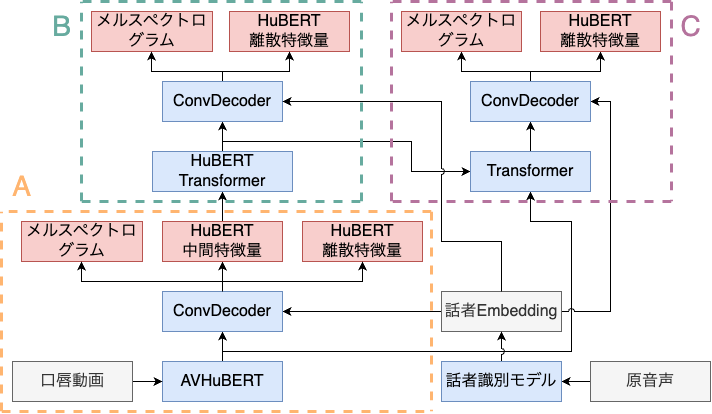
\includegraphics[height=90mm]{./figure/sec4/model/network.png}
    \caption{ネットワークの概略図}
    \label{sec4:fig:network}
\end{figure}

\begin{figure}[bt]
    \centering
    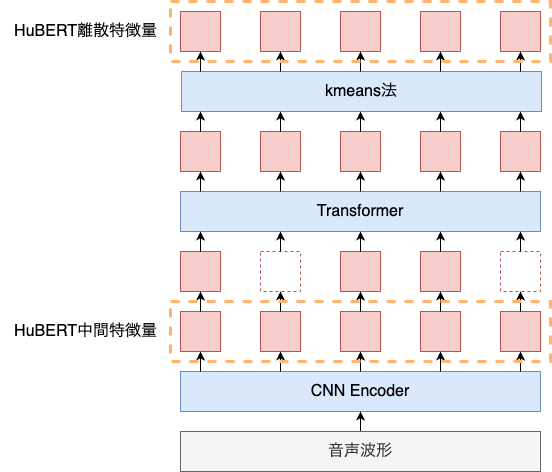
\includegraphics[height=90mm]{./figure/sec4/model/hubert.png}
    \caption{HuBERT中間特徴量とHuBERT離散特徴量の概略}
    \label{sec4:fig:hubert}
\end{figure}

三段階目では、二段階目までに学習されたネットワークAとネットワークBの重みを固定した状態で、AVHuBERTから得られる特徴量と、HuBERT Transformer層から得られる特徴量の二つを結合し、それらを入力として再びメルスペクトログラムとHuBERT離散特徴量の予測を行うネットワークCを学習した(図~\ref{sec4:fig:network}のC)。ネットワークCでは、はじめに前述した二つの特徴量をチャンネル方向に結合することで、1536次元の入力特徴量を得る。これに対して全結合層を施すことで再度768次元に圧縮し、4層のTransformer層を通すことで系列全体を考慮した特徴抽出を改めて行った。その後、ネットワークA,Bと同様に話者Embeddingを結合し、ConvDecoderを通すことによって予測値を得た。ここで、ネットワークCのTransformer層におけるパラメータについては、AVHuBERTやHuBERTと同様にチャンネル数を768、ヘッド数は12とした。ネットワークCの役割は、ネットワークBと同様に音声波形への変換に必要な特徴量の予測である。ここでの狙いについて、まず、AVHuBERTから得られる特徴量とHuBERT Transformer層から得られる特徴量は、どちらもConvDecoderへの入力となる点で同じである。一方、AVHuBERTは動画を入力、HuBERT Transformer層はHuBERT中間特徴量を入力とするため、これら特徴量の元となる入力は異なっている。ここでは、概ね同じ予測対象のために利用される二つの特徴量(ネットワークAではHuBERT中間特徴量の予測も行っているため、全く同じではない)が、入力の違いに依存して内部のSelf Attentionにより注意される部分が変化し、何らかの異なった情報を持っている可能性があると仮定した。この仮定に基づき、両方の特徴量を考慮して単一特徴量への依存を解消することで、汎化性能向上による予測精度の改善を狙った。

以上が提案手法の全体像であるが、今回ベースラインとする先行研究\cite{choi2023intelligible}に基づいたマルチタスク学習手法は、本研究におけるネットワークAで、HuBERT中間特徴量を推定しないものに当たる。AVHuBERT以降のConvDecoderについて、これは先行研究と異なる構成であるが、これは実験の過程でより良いものを選択した結果である。本実験においてはこれを比較手法全てで一貫して用いることで、比較したい部分には影響が出ないようにしつつ、全体的な性能の底上げを狙った。

以上のモデルにより、動画からメルスペクトログラムとHuBERT離散特徴量が推定可能となる。その後、先行研究~\cite{choi2023intelligible}に基づくMulti-input Vocoderを用い、メルスペクトログラムとHuBERT離散特徴量を入力として音声波形に変換することで、最終的な合成音声を得た。Multi-input VocoderはHiFi-GAN~\cite{kong2020hifi}をベースとしたモデルであり、音声波形を生成するGeneratorと、Multi Scale DiscriminatorおよびMulti Period Discriminatorという二つのDiscriminatorによって構成される。Generatorへの入力特徴量について、メルスペクトログラムは100Hz、HuBERT離散特徴量は50Hzとなっているが、メルスペクトログラムは隣接したフレームを次元方向に縦積みすることで、100Hz・80次元の特徴量から50Hz・160次元の特徴量に変換して用いた。入力時は全結合層によって128次元の特徴量に変換した。一方、HuBERT離散特徴量はインデックス系列であるが、入力時はインデックスから128次元のベクトルに変換した。その後、これらをチャンネル方向に結合することで256次元の特徴量を構成し、これをGeneratorへの最終的な入力とした。その後は、HiFi-GANの公式実装と同様である。

\subsection{実験方法}
\subsubsection{利用したデータセット}
動画音声データセットには、男女二人ずつから収録した合計4人分のデータセット~\cite{taguchi,esaki}を用いた。これはATR音素バランス文~\cite{atr}から構成され、全話者共通でAからHセットを学習データ、Iセットを検証データ、Jセットをテストデータとして利用した。各分割ごとの文章数を表~\ref{sec4:tab:dataset_info}に示す。

Multi-input Vocoderの学習に利用する音声データセットには、Hi-Fi-Captain(日本語話者二名分)~\cite{okamoto2023hi}とJVS(parallel100とnonpara30)~\cite{takamichi2019jvs}を利用した。ボコーダの学習時にはサンプル全体から1秒分をランダムにサンプリングして用いるが、元データには話し声のない無音区間が一定存在しており、これはボコーダの学習に望ましくない。これに対して、無音区間のトリミング(-40 dBFS未満かつ500 ms継続する区間を100 msまでカット)を適用した。Hi-Fi-Captainはtrain-parallelおよびtrain-non-parallelを学習データ、valを検証データ、evalをテストデータとして分割した。各分割ごとの文章数を表~\ref{sec4:tab:dataset_info}に示す。JVSには話者に対して1から100まで番号が割り振られており、本実験では1から80番の話者を学習データ、81番から90番の話者を検証データ、91番から100番までの話者をテストデータとした。各分割ごとの文章数を表~\ref{sec4:tab:dataset_info}に示す。

\begin{table*}[bt]
    \centering
    \caption{利用したデータセットの文章数}
    \label{sec4:tab:dataset_info}
    \begin{center}
        \renewcommand{\arraystretch}{0.9} % 行の高さ調整
        \setlength{\tabcolsep}{8pt}      % 列の幅調整
        \scalebox{1.0}{
            \begin{tabular}{|l|r|r|r|}
                \hline
                              & \multicolumn{1}{c|}{学習} & \multicolumn{1}{c|}{検証} & \multicolumn{1}{c|}{テスト} \\
                \hline
                動画音声データセット    & 1598                    & 200                     & 212                      \\
                Hi-Fi-Captain & 37714                   & 200                     & 200                      \\
                JVS           & 10398                   & 1299                    & 1300                     \\
                \hline
            \end{tabular}
        }
    \end{center}
\end{table*}

\subsubsection{データの前処理}
動画データは60 FPSで収録されたものをffmpegにより25 FPSに変換して用いた。その後、手法~\cite{bulat2017far}により動画に対してランドマーク検出を適用した。このランドマークを利用することで口元のみを切り取り、画像サイズを(96, 96)にリサイズした上で、グレースケールに変換した。加えて、画像に対する正規化および標準化を適用した。全体として、今回は事前学習済みのAVHuBERTの転移学習を行うため、そこでの前処理に合わせている。学習時は、ランダムクロップ、左右反転、Time Masking(一時停止)をデータ拡張として適用した。ランダムクロップは、(96, 96)で与えられる画像から(88, 88)をランダムに切り取る処理である。検証およびテスト時は、必ず画像中央を切り取るよう実装した。左右反転はランダムクロップ後に適用しており、50\%の確率で左右が反転されるよう実装した。Time Maskingは、連続する画像の時間平均値を利用することによって、一時停止させるような効果を与えるデータ拡張手法である。動画1秒あたり0から0.5秒の間でランダムに停止区間を定め、その区間における動画の時間方向平均値を計算し、区間内のすべてのフレームをこの平均値で置換した。

音声データは48 kHzで収録されたものを16 kHzにダウンサンプリングして用いた。それから、窓長25 msのハニング窓を用いて、シフト幅10 msでSTFTを適用することでフレームレート100 Hzのスペクトログラムに変換した。さらに、振幅スペクトログラムに対して80次のメルフィルタバンクを適用し、メルスペクトログラムを得た上で対数スケールに変換した。話者Embeddingの取得には事前学習済みの話者識別モデル~\cite{wan2018generalized}を利用し、学習データから100個ランダムサンプリングして計算した平均値を利用した。

HuBERTは、HuggingFaceに公開されているReazonSpeechというデータセットによって学習されたモデル~\cite{rinna-japanese-hubert-base,sawada2024release}を利用した。ReazonSpeechは約19000時間の日本語音声からなるデータセットであり、日本語音声のコンテキストを大量のデータから学習したモデルである。今回用いるデータセットが日本語であることから、本研究の検討対象としては日本語音声に関する事前知識を豊富に有するモデルが適していると考え、このモデルを選択した。動画からの予測対象となるHuBERT離散特徴量は、k-means法によるクラスタリング(クラスタ数100)をHuBERT Transformer層の8層目出力に適用することで得た。8層目を選択した理由は、HuBERTのレイヤーごとの特徴量について、音素のOne-hotベクトルおよび単語のOne-hotベクトルとの相関を、Canonical Correlation Analysis(CCA)によって調べた先行研究\cite{pasad2023comparative}より、8層目出力がそのどちらとも相関が高く言語的な情報に近いと判断したからである。k-means法の学習には動画音声データセットにおける学習用データを利用し、これによって動画音声データおよび、Multi-input Vocoderの学習に用いる外部の音声データについてクラスタリングを適用した。

\subsubsection{学習方法}
一段階目について、損失関数はメルスペクトログラムのMAE Loss $L_{mel}$ とHuBERT離散特徴量のCross Entropy Loss $L_{ssl^{d}}$ 、HuBERT中間特徴量のMAE Loss $L_{ssl^{i}}$ の重み付け和とした。それぞれの重み係数を$\lambda_{mel}, \lambda_{ssl^{d}}, \lambda_{ssl^{i}}$とすると、
\begin{equation}
    \label{sec4:eq:loss}
    L = \lambda_{mel} * L_{mel} + \lambda_{ssl^{d}} * L_{ssl^{d}} + \lambda_{ssl^{i}} * L_{ssl^{i}}
\end{equation}
となる。第一段階では$\lambda_{mel} = 1.0, \lambda_{ssl^{i}} = 1.0$と固定し、$\lambda_{ssl^{d}}$のみ0.0001から1.0まで10倍刻みで5段階試してチューニングを行った。最適化手法にはAdamW~\cite{loshchilov2017decoupled}を利用し、$\beta_{1} = 0.9$、$\beta_{2} = 0.98$、$\lambda = 0.01$とした。学習率は\num{1.0e-3}から開始し、Warmup Schedulerによってその値を変化させた。バッチサイズはメモリの都合上4としたが、学習の安定のためGradient Accumulationによって各イテレーションにおける勾配を累積させ、8イテレーションに一回重みを更新するようにした。そのため、実質的にはバッチサイズ32となる。モデルに入力する動画の秒数は10秒を上限とし、それを超える場合はランダムにトリミング、それに満たない場合はゼロパディングした。勾配のノルムは3.0を上限としてクリッピングすることで、過度に大きくなることを防止した。最大エポック数は50とし、10エポック連続して検証データに対する損失が小さくならない場合には、学習を中断するようにした(Early Stopping)。また、学習終了時には検証データに対する損失が最も小さかったエポックにおけるチェックポイントを保存し、これをテストデータに対する評価に用いた。

第二段階について、損失関数はメルスペクトログラムのMAE LossとHuBERT離散特徴量のCross Entropy Lossの重み付け和とした。これは式~\eqref{sec4:eq:loss}において、$\lambda_{mel} = 1.0, \lambda_{ssl^{i}} = 0.0$と固定した場合に相当する。第一段階と同様に、$\lambda_{ssl^{d}}$のみ0.0001から1.0まで10倍刻みで5段階試してチューニングを行った。最適化手法にはAdamWを利用し、$\beta_{1} = 0.9$、$\beta_{2} = 0.98$、$\lambda = 0.01$とした。学習率は\num{5.0e-4}から開始し、Warmup Schedulerによってその値を変化させた。学習率について第一段階と異なるが、これは値を半減させることによって学習を安定させることができたためである。その他のパラメータは、第一段階における値と同じである。

第三段階について、学習率のみ第一段階と同様に\num{1.0e-3}としたが、それ以外は第二段階と全く同じである。

Multi-input Vocoderの学習について、学習は動画音声データセットではなく、外部データであるHi-Fi-CaptainとJVSを用いた。はじめにHi-Fi-Captainのみを用いて学習させ、その後学習済みモデルをJVSによって再学習した。Hi-Fi-Captainは男女一人ずつの文章数が豊富なデータセットであるため、高品質なモデルを構築可能であった。しかし、学習できる話者数が少ない分、学習外話者に対する合成音声の品質が低かった。そのため、一人当たりの文章数は100文章程度と少ないながらも、100人分の話者からなるJVSを利用して再学習することによって、学習外話者に対する合成音声の品質を向上させた。最適化手法にはAdamWを利用し、$\beta_{1} = 0.8$、$\beta_{2} = 0.99$、$\lambda = 0.01$とした。学習率は\num{2.0e-4}から開始し、指数関数的にその値を変化させた。バッチサイズは16とし、ここではGradient Accumulationは利用しなかった。モデルへの入力は1秒を上限とし、それを超える場合はランダムにトリミング、それに満たない場合はゼロパディングした。勾配のノルムは3.0を上限としてクリッピングすることで、過度に大きくなることを防止した。最大エポック数は30とし、ここではEarly Stoppingは適用しなかった。また、学習終了時には検証データに対する損失(メルスペクトログラムに対するL1 Loss)が最も小さかったエポックにおけるチェックポイントを保存し、これをテストデータに対する評価に用いた。また、Multi-input Vocoderの提案された先行研究~\cite{choi2023intelligible}においては、学習時にあえてメルスペクトログラムにノイズをかけることによって、合成音声に対する汎化性能を向上させる学習方法が提案されている。本研究では、動画から推定されるメルスペクトログラムとHuBERT離散特徴量の推定精度向上に焦点を当てたため、Multi-input Vocoderの学習は原音声から計算される特徴量そのもので行い、ボコーダ自体の汎化性能向上による精度改善は追求しなかった。

実装に用いた深層学習ライブラリはPyTorchおよびPyTorch Lightningである。GPUにはNVIDIA RTX A4000を利用し、計算の高速化のためAutomatic Mixed Precisionを適用した。

\subsubsection{比較手法}
\label{sec4:subsubsection:methods}
比較手法は、以下の五つである。
\begin{enumerate}
    \item メルスペクトログラムとHuBERT離散特徴量のマルチタスク学習手法(ベースライン)
    \item 提案手法のネットワークBで、ランダム初期化したHuBERT Transformer層を用いる手法
    \item 提案手法のネットワークCで、ランダム初期化したHuBERT Transformer層を用いる手法
    \item 提案手法のネットワークBで、事前学習済みのHuBERT Transformer層を用いる手法
    \item 提案手法のネットワークCで、事前学習済みのHuBERT Transformer層を用いる手法
\end{enumerate}
手法1が先行研究において有効性が確認された手法であり、今回の実験においてベースラインとなる。これに対する改善案として、手法2から手法5が提案手法である。手法2および手法3は、今回期待するHuBERTの事前学習済み重みを初期値とした転移学習が本当に有効であるか検証する目的で、あえてランダム初期化したHuBERT Transformerを用いる場合である。

\subsubsection{客観評価}
合成音声の客観評価では、二種類の指標を用いた。
一つ目は、音声認識の結果から算出したWord Error Rate(WER)である。Whisper~\cite{radford2023robust}を用いて音声認識を行い、出力される漢字仮名交じり文に対してMeCabを用いて分かち書きを行った上で、jiwerというライブラリを用いて算出した。WhisperはLargeモデルを利用し、MeCabの辞書にはunidicを利用した。WERの値は0\%から100\%であり、この値が低いほど音声認識の誤りが少ないため、より聞き取りやすい音声であると判断した。
二つ目は、話者Embeddingから計算したコサイン類似度である。話者Embeddingの計算は、モデルへの入力値を計算したものと同様の話者識別モデルを利用し、対象音声と原音声のペアでコサイン類似度を計算した。今回構築するモデルは4人の話者に対応するモデルとなるため、原音声に似た声質の合成音声が得られているかをこの指標で評価した。値は0から1であり、高いほど原音声と類似した合成音声だと判断できる。

\subsubsection{主観評価}
合成音声の主観評価では、音声の明瞭性と類似性の二点を評価した。今回はクラウドワークスというクラウドソーシングサービスおよび、自作の実験用Webサイトを利用してオンラインで実験を実施した。被験者の条件は、日本語母語話者であること、聴覚に異常がないこと、イヤホンあるいはヘッドホンを用いて静かな環境で実験を実施可能であることとした。被験者の方に行っていただいた項目は、以下の五つである。
\begin{enumerate}
    \item アンケート
    \item 練習試行(明瞭性)
    \item 本番試行(明瞭性)
    \item 練習試行(類似性)
    \item 本番試行(類似性)
\end{enumerate}

一つ目のアンケートでは、被験者についての基本的な統計を取ることを目的として、性別・年齢・実験に利用した音響機器について回答してもらった。性別は、男性、女性、無回答の三つからの選択式とした。年齢は被験者の方に直接数値を入力してもらう形式とした。実験に使用した音響機器は、イヤホン、ヘッドホンの二つからの選択式とした。

二つ目の練習試行(明瞭性)および三つ目の本番試行(明瞭性)では、音声の明瞭性の評価を実施した。初めに練習試行を行っていただくことで実験内容を把握してもらい、その後本番施行を行っていただく流れとした。ここで、練習施行は何度でも実施可能とし、本番試行は一回のみ実施可能とした。
評価項目について、明瞭性は「話者の意図した発話内容をその通り聞き取ることができるか」を評価するものとした。実際の評価プロセスは以下の三段階で構成した。
\begin{enumerate}
    \item 音声サンプルのみを聞いてもらい、その音声の発話内容を聞き取ってもらう。
    \item 発話内容を聞き取ることができた、あるいはこれ以上聞き取ることはできないと判断したら、本来の発話内容を確認してもらう。
    \item 聴取者が想定していた発話内容と本来の発話内容を照らし合わせ、音声の聞き取りやすさを5段階評価してもらう。
\end{enumerate}
5段階評価の回答項目は以下のようにした。
\begin{enumerate}
    \item 全く聞き取れなかった
    \item ほとんど聞き取れなかった
    \item ある程度聞き取れた
    \item ほとんど聞き取れた
    \item 完全に聞き取れた
\end{enumerate}

実験に利用した音声サンプルについて、練習試行では検証データ、本番試行ではテストデータを用いた。評価対象とした音声の種類は、\ref{sec4:subsubsection:methods}節における五つの手法と、原音声、分析合成を加えた7種類である。被験者ごとの評価サンプルの割り当て方法について、初めに評価に用いる文章を比較手法の総数である7つのグループにランダムに分割した。具体的には、練習試行では検証データであるATR音素バランス文のIセットから7種類、本番試行ではテストデータであるATR音素バランス文のJセットのすべて、すなわち53種類の文章を7つの文章グループにランダムに分割した。次に、各文章グループに対して7種類の手法から一つを割り当てることで、文章一つ一つに対する手法の割り当てを行った。残る話者の決定については、ランダムに割り当てるようにした。文章グループに対して割り当てる手法は、被験者ごとにずらすよう実装した。この過程を表~\ref{sec4:tab:sbj_selection_relation}に示す。これは、7つの文章グループに対し、割り当てる手法が一つずつずれていく過程を表している。これにより、文章と手法の組み合わせを効率よく網羅できる\cite{king2008blizzard}。またこの選択方法により、各話者はすべての文章を一回ずつ評価する機会が与えられ、その中で各手法がなるべく均等な回数含まれることとなる。同じ発話内容の音声を二回以上提示しないことで、聴取者の集中力を保つことを狙った。また、各手法をなるべく均等な回数提示するようにした理由は、手法の比較が主観評価の最終的な目的であったため、各被験者がすべての手法を評価する機会を与えたかったからである。
加えて、サンプル選択の過程では、以前に選択された回数をカウントしておくことで、サンプルの選択にランダム性を持たせつつ、すべてのサンプルが等しい回数評価されるようにした。例えば、一回選択されたサンプルと未選択のサンプルが存在する場合、一回選択されたサンプルは選択の候補から除外する。これにより、未選択のサンプルのみを対象としたランダムサンプリングを行うことで、最終的な評価回数が等しくなるよう実装した。本実験では手法が七種類、話者が四人存在するため、28回の実験によって、手法・話者・文章のすべての組み合わせが一回ずつ評価される、すなわち全サンプルが一回ずつ評価されることになる。

\begin{table*}[bt]
    \centering
    \caption{主観評価実験のサンプル選択における文章グループと手法の対応関係}
    \label{sec4:tab:sbj_selection_relation}
    \begin{center}
        \renewcommand{\arraystretch}{1.0} % 行の高さ調整
        \setlength{\tabcolsep}{8pt}      % 列の幅調整
        \scalebox{0.9}{
            \begin{tabular}{|c|ccccccc|}
                \hline
                \multirow{2}{*}{}         & \multicolumn{7}{c|}{文章グループインデックス}                         \\
                                          & 1                                 & 2 & 3 & 4 & 5 & 6 & 7 \\
                \hline
                \multirow{7}{*}{手法インデックス} & 1                                 & 2 & 3 & 4 & 5 & 6 & 7 \\
                                          & 2                                 & 3 & 4 & 5 & 6 & 7 & 1 \\
                                          & 3                                 & 4 & 5 & 6 & 7 & 1 & 2 \\
                                          & 4                                 & 5 & 6 & 7 & 1 & 2 & 3 \\
                                          & 5                                 & 6 & 7 & 1 & 2 & 3 & 4 \\
                                          & 6                                 & 7 & 1 & 2 & 3 & 4 & 5 \\
                                          & 7                                 & 1 & 2 & 3 & 4 & 5 & 6 \\
                \hline
            \end{tabular}
        }
    \end{center}
\end{table*}

四つ目の練習試行(類似性)および五つ目の本番試行(類似性)では、評価対象の音声と同一話者の原音声の類似性の評価を実施した。ここでも初めに練習試行を行っていただくことで実験内容を把握してもらい、その後本番施行を行っていただく流れとした。ここで、練習施行は何度でも実施可能とし、本番試行は一回のみ実施可能とした。
評価項目について、類似性は「評価対象の音声が同一話者の原音声とどれくらい似ているか」を評価するものとした。実際の評価プロセスは以下の二段階で構成した。
\begin{enumerate}
    \item 評価対象の音声と原音声を聞き比べてもらう。
    \item 評価対象の音声が原音声にどれくらい似ていたかを五段階評価してもらう。
\end{enumerate}
5段階評価の回答項目は以下のようにした。
\begin{enumerate}
    \item 全く似ていなかった
    \item あまり似ていなかった
    \item やや似ていた
    \item かなり似ていた
    \item 同じ話者に聞こえた
\end{enumerate}
実験に利用した音声サンプルおよび、被験者ごとの評価サンプルの割り当て方法は明瞭性の評価実験と同様である。ただし、類似性評価においては同一話者の原音声を発話内容についてランダムに選択し、評価対象となるサンプルとペアで提示できるようにした。評価時は、明瞭性評価と同様に音声サンプルを何度でも聞けるようにしたが、発話文章については提示しなかった。なぜなら、類似性評価では評価が発話文章に依存しないからである。実際、評価サンプルのペアとなる原音声サンプルは発話文章をランダムに選択しているため、一致する場合も異なる場合も存在する。

また、オンラインでの評価は効率よく数多くの方に評価していただけるという点でメリットがあるが、オフラインでの評価と比較して実験環境を制御することが難しく、評価品質が低下する恐れがある。これに対して、本実験では先行研究\cite{kirkland2023stuck}を参考に、評価サンプル中にダミー音声を混入させることで対策を講じた。ダミー音声は本研究で得られた合成音声とは無関係に、gTTSというライブラリを用いて生成したサンプルである。具体例として、明瞭性評価では
\begin{quote}
    これはダミー音声です。明瞭性は「3: ある程度聞き取れた」を選択してください。
\end{quote}
のような発話内容の音声を、類似性評価では
\begin{quote}
    これはダミー音声です。類似性は「1: 全く同じ話者には聞こえなかった」を選択してください。
\end{quote}
のような発話内容の音声を提示した。この時、その音声自体の明瞭性や類似性とは無関係に、必ずこの音声によって指定された評価値を選択するよう説明を与えた。本番試行においてダミー音声で指定された評価値を誤って選んだ場合は、すべての回答を無効にする旨を被験者に伝えた。実際、実験終了後にはそのようにデータを処理した。

被験者数および各手法の評価回数に関して、先行研究\cite{wester2015we}では主観評価実験の結果に対する統計処理について、そこで用いる被験者数や手法ごとの評価回数を変数とし、実験条件に対してどれほどの被験者数とサンプル数が必要そうであるかを検討している。今回はこの研究を参考にしつつ、オンラインで実験を実施するのであれば総被験者数が100人以上、各手法に対する総評価回数が200回以上となることが望ましいと判断した。前述した各被験者に対するサンプルの選択方法により、28回の実験によって全てのサンプルが一回ずつ評価される。これを1セットとすると、セットあたり被験者数は28人、各手法に対する評価回数は212回となる。従って、今回は4セット行うことで、総被験者数112人、各手法に対しての総評価回数が848回となるようにした。実験は30分程度で終わると見積もって、一人当たりの報酬は500円とした。

\subsection{結果}
\subsubsection{客観評価}
まず、損失関数~\eqref{sec4:eq:loss}の重み係数$\lambda_{ssl^{d}}$を変化させた時の、客観評価指標の全テストデータに渡る平均値を表~\ref{sec4:tab:obj_weights}に示す。各手法ごとに0.0001から1.0まで10倍刻みで5段階検討し、各手法の客観指標ごとに最も優れた値を下線で示している。最良エポックは検証データに対する損失が最小となったエポックであり、テストデータの合成にはこのエポックにおけるチェックポイントを利用した。また、$L_{mel}$、$L_{ssl^{d}}$、$L$は最良エポックにおける検証データに対する損失の平均値である。また、これ以降の比較のために、最適だと考えられる$\lambda_{ssl^{d}}$の値を選択しており、選択された行を太字で表している。

手法1では、$\lambda_{ssl^{d}}$の値が0.0001の時にWERが最も低く、0.01の時に話者類似度が最も高くなった。現状WERの高さが特に課題であり、話者類似度は0.004とわずかな違いでもあるため、今回はWERが最小であることを優先して0.0001が最適であると判断した。$\lambda_{ssl^{d}}$の値による評価指標の変化について、WERは$\lambda_{ssl^{d}}$の値を大きくするのに伴って単調に増加していることがわかる。一方、話者類似度は$\lambda_{ssl^{d}}$の値が0.1以上となった時に、0.01以下であった場合と比較して顕著に低下することがわかる。次に、図~\ref{sec4:fig:learning_curve_method_1_val_losses}に手法1における学習曲線の結果を示す。横軸がエポック数、縦軸が損失の値を表す。損失の値は各エポックにおける平均値である。実線は検証データに対する損失、点線は学習データに対する損失を表しており、線の色は$\lambda_{ssl^{d}}$の違いを表す。また、丸いマーカーは表~\ref{sec4:tab:obj_method_comp}に示した最良エポック時における損失の値を表す。学習曲線より、$\lambda_{ssl^{d}}$の値を変化させることによって、特に$L_{ssl^{d}}$の傾向が変化していることがわかる。具体的には、$\lambda_{ssl^{d}}$の値を0.0001から1.0へと増加させるのに伴って、学習初期における損失の下がり方が急峻になっており、達する最小値自体が小さくなっていることがわかる。また、$\lambda_{ssl^{d}}$の値が0.1以上の場合、検証データに対する$L_{ssl^{d}}$は早いうちから増加傾向に転じている。これに伴い、今回は検証データに対する$L$の値を監視し、Early Stoppingの適用と最良エポックの決定を行なったため、$L_{mel}$が下がり切らない状態で学習が中断される結果となった。客観評価指標において、特に$\lambda_{ssl^{d}}$の値が0.1以上となるとき、0.01以下の場合と比較して話者類似度の低下や、WERの上昇傾向が見られていたが、学習曲線の挙動より、$L_{mel}$を下げきれなくなっていたことが原因として考えられる。最適な$\lambda_{ssl^{d}}$の値は客観評価指標から0.0001としたが、0.01以下ではそれと概ね同程度の品質であったことを考えると、手法1では検証データに対する$L_{mel}$の値を十分小さくすることのできる$\lambda_{ssl^{d}}$が適していると考えられる。

手法2では、$\lambda_{ssl^{d}}$の値が0.1の時にWERが最も低く、0.0001の時に話者類似度が最も高くなった。ここでは$\lambda_{ssl^{d}}$の値が0.1の時に、ベースラインで選択された最適なケースと比較してWERが9.1\%低下しており、話者類似度についても0.003高くなっていることから、0.1が最適だと判断した。$\lambda_{ssl^{d}}$の値による評価指標の変化について、$\lambda_{ssl^{d}}$を0.1以上とすることで、0.01以下の場合と比較してWERが低下する傾向が見られた。しかし、1.0まで大きくすると0.1の場合よりもWERが大きくなっており、単調に減少していないこともわかる。話者類似度については、$\lambda_{ssl^{d}}$の値を0.1としたときに、0.01以下の場合と比較して値が少し低下し、さらに1.0まで大きくすることで0.1以下の場合と比較して顕著に低下していることがわかる。次に、図~\ref{sec4:fig:learning_curve_method_2_val_losses}に手法2における学習曲線の結果を示す。手法1と同様に、$\lambda_{ssl^{d}}$の値を0.0001から1.0へと増加させるのに伴って、学習初期における$L_{ssl^{d}}$の下がり方が急峻になっており、達する最小値自体が小さくなっていることがわかる。また、$\lambda_{ssl^{d}}$が1.0の場合に、$L_{mel}$を下げきれなくなる傾向が見られる。加えて、手法2では$\lambda_{ssl^{d}}$が0.1の場合における$L_{ssl^{d}}$の増加が緩やかであり、$L_{mel}$も十分下げられていることがわかる(ただし、表~\ref{sec4:tab:obj_weights}の$L_{ssl^{d}}$より、手法1の$\lambda_{ssl^{d}}$が0.1の場合と比較して、損失の値自体は大きい)。さらに、$\lambda_{ssl^{d}}$が0.1の場合、$L_{mel}$が達する最小値自体が、$\lambda_{ssl^{d}}$が0.01以下の場合と比較して小さくなっていることがわかる(具体的な値は表~\ref{sec4:tab:obj_weights}の$L_{mel}$の値を参照)。これは手法1では見られなかった新たな傾向であった。最適な$\lambda_{ssl^{d}}$の値は客観評価指標から0.1としたが、学習曲線の挙動より、この時他の値の場合と比較して$L_{mel}$と$L_{ssl^{d}}$の両方をバランスよく下げられていたことがわかった。よって、手法2においては$L_{mel}$と$L_{ssl^{d}}$の両方をバランスよく下げられるような、程よい大きさの重みが適していると考えられる。

手法3における最適値の選択理由は手法2と同様であり、$\lambda_{ssl^{d}}$の値による評価指標の変化についても同様であった。次に、図~\ref{sec4:fig:learning_curve_method_3_val_losses}に手法3における学習曲線の結果を示す。傾向は手法2と概ね同様であるが、手法3では$\lambda_{ssl^{d}}$の値が0.1の場合における$L_{ssl^{d}}$の増加が早く、学習が早期に中断されている点は異なる。しかし、この時$L_{mel}$も十分下げられており、$L_{mel}$が達する最小値自体が、$\lambda_{ssl^{d}}$が0.01以下の場合と比較して小さくなっていることがわかる(具体的な値は表~\ref{sec4:tab:obj_weights}の$L_{mel}$の値を参照)。以上より、細かな違いはあるものの手法3は手法2と同様の挙動を示し、$\lambda_{ssl^{d}}$は$L_{mel}$と$L_{ssl^{d}}$の両方をバランスよく下げられるような、程よい大きさの重みが適していると考えられる。

手法4及び手法5についても、最適値の選択理由は手法2と同様である。しかし、これらは$\lambda_{ssl^{d}}$の値を0.1としたときの話者類似度の低下の度合いが手法2、手法3と比較して大きい点で、傾向が異なっていた。次に、図~\ref{sec4:fig:learning_curve_method_4_val_losses}に手法4、図~\ref{sec4:fig:learning_curve_method_5_val_losses}に手法5における学習曲線の結果を示す。傾向については、$L_{ssl^{d}}$の増加の程度について細かな違いはあるが、概ね手法2と同様であり、$L_{mel}$と$L_{ssl^{d}}$の両方をバランスよく下げられるような、程よい大きさの重みが適していると考えられる。また、手法4と手法5において、$\lambda_{ssl^{d}}$が0.1の場合における話者類似度は、手法2および手法3と比較して低くなっていたが、$L_{mel}$や$L_{ssl^{d}}$の値からは一貫した傾向が見られない。これより、平均値からこの違いを分析することは難しいが、実際の細かな誤差の出方が異なっていて、これが影響を与えているのではないかと考える。

次に、最適なチューニングをした場合における、手法ごとの客観評価指標の全テストデータに渡る平均値を表~\ref{sec4:tab:obj_method_comp}に示す。分析合成は、原音声から計算した特徴量を入力として、Multi-input Vocoderで逆変換した合成音声であり、本実験下において合成音声により達成され得る上限値を表す。手法1から手法5については、表~\ref{sec4:tab:obj_weights}において太字としたもの、すなわち最適なチューニングだと判断されたものを選択している。また、分析合成、原音声を除いた合成音声(手法1から手法5)の中で、最も優れた値を下線で示している。
これより、WER、話者類似度ともに手法3が最も優れていることが分かる。特に、今回のベースラインである手法1と比較すると、WERが9.5\%低下し、話者類似度は0.01高くなっていることから、提案手法がベースラインよりもより聞き取りやすく、話者性を反映した音声を合成できたと考えられる。
また、HuBERTの事前学習済み重みを初期値とすることの効果について、手法2と手法4を比較すると、手法2の方がWERが1.2\%低く、話者類似度が0.017高いことがわかる。よって、本研究ではHuBERTの事前学習済み重みを初期値とした転移学習が有効である可能性を検討したが、むしろ事前学習済み重みを初期値とせず、ランダム初期化したモデルの方が優れていたと考えられる。これは仮説に反した結果であったが、事前学習済み重みによって与えられる初期値が、より良い局所解への収束には繋がらなかったことが原因だと考えられる。一方、アンサンブル手法の有効性について、手法2と手法3を比較すると、アンサンブル手法を導入することによってWERが0.4\%低下し、話者類似度が0.007高くなっていることから、わずかではあるが改善していることがわかる。しかし、手法4と手法5を比較すると、WERは変化せず、話者類似度は0.017低下していることから、特に話者類似度の観点で悪化したことがわかる。よって、アンサンブル手法は必ずしも改善につながるわけではなく、改善するとしても顕著な変化はもたらさないと考えられる。

次に、最適なチューニングをした場合における手法ごとに、発話文章ごとのWERの比較を行った結果を図~\ref{sec4:fig:wer_sample_wise_comparison}に示す。ここで、縦軸は発話文章を表し、横軸はベースラインである手法1とその他手法の間でWERの差を計算し、発話文章ごとに平均した値を表す。負の値を取っているとき、手法1に対してより低いWERを達成したと解釈できる。図より、表~\ref{sec4:tab:obj_method_comp}における平均値のみを見れば、手法2から手法5の全てが手法1に対してより低いWERを達成していたが、発話文章ごとに見れば、手法1に対してWERが高くなっているサンプルもあることがわかる。例えば、「ATR503\_j11」では、手法2から手法5の全てがベースラインよりも20\%前後高いWERとなっていることがわかる。また、全体的な傾向として手法ごとにWERはばらけており、いかなる場合においても最良となるようなモデルは構築できていないことがわかる。これより、現状のいかなるモデルも発話文章に対する汎化性能が不十分であり、さらなる改善が必要だと考えられる。

次に、話者ごとのWERの比較を行った結果を図~\ref{sec4:fig:wer_speaker_wise_comparison}に示す。ここで縦軸は話者を表し、横軸はベースラインである手法1とその他手法の間でWERの差を計算し、話者ごとに平均した値を表す。負の値を取っているとき、手法1に対してより低いWERを達成したと解釈できる。これより、手法2から手法5は平均的にいかなる話者に対しても手法1より低いWERを達成していることがわかるが、一方でその改善の度合いは話者によって異なることがわかる。特に、「F02\_kablab」はその他三人の話者と比較して改善の度合いが小さい。また、例えば「F01\_kablab」では手法2と手法3がより有効である一方、「F02\_kablab」では手法4と手法5がより有効となっており、有効な手法が話者によって異なることもわかる。これより、話者に対する性能の依存があると考えられ、さらなる汎化性能の向上が必要だと言える。

次に、話者ごとの話者類似度の比較を行った結果を図~\ref{sec4:fig:spk_sim_speaker_wise_comparison}に示す。ここで縦軸は話者を表し、横軸はベースラインである手法1とその他手法の間で話者類似度の差を計算し、話者ごとに平均した値を表す。正の値を取っているとき、手法1に対してより高い話者類似度を達成したと解釈できる。これを見ると、手法4と手法5はいかなる話者に対しても話者類似度を悪化させたことがわかる。手法4と手法5は事前学習済み重みを初期値としたモデルであったため、この影響が出ている可能性がある。今回検討したHuBERTは音声の言語情報を考慮する点で強みがあり、実際音声認識ではその転移学習の有効性が確認されている。しかし、話者性を考慮するという点で特に有効でなく、話者性を軽視するような局所解への収束に繋がった可能性が考えられる。ただ、表~\ref{sec4:tab:obj_weights}より手法4と手法5においても$\lambda_{ssl^{d}}$が0.01以下であれば、比較的高い話者類似度を達成していたため、損失の重み付けにも依存していると言える。また、手法3はいかなる話者に対しても類似度を向上させており、この点で優れていたと言える。手法2では「F02\_kablab」のみ話者類似度が悪化しており、手法3と比較して話者に対する汎化性能が低かったと考えられる。

以上のことから、提案手法である手法2から手法5はいずれも手法1に対して平均的にWERを低下させ、特に手法2及び手法3は話者類似度についても若干の改善を達成したことから、提案手法によるベースラインからの改善が達成できたと考える。また、HuBERTの事前学習済み重みを用いることは仮説に反して有効ではなく、アンサンブル手法についてもその効果は顕著なものではなかった。さらに、特に手法2から手法5は損失関数の重み係数である$\lambda_{ssl^{d}}$による性能の変化が著しく、ここで最適値を選択できなければベースラインである手法1から改善しないこともわかった。よって、提案手法におけるベースラインからの改善に寄与した可能性のあるポイントは、以下でまとめられる。
\begin{enumerate}
    \item HuBERT中間特徴量を入力とし、メルスペクトログラムとHuBERT離散特徴量を推定するネットワークを導入したこと
    \item 上記のネットワーク構造をHuBERT Transformerとしたこと
    \item ネットワークをランダム初期化した上で学習させたこと
    \item 最適な$\lambda_{ssl^{d}}$の値を発見できたこと
\end{enumerate}
本実験からは、HuBERT Transformerをランダム初期化する必要性と、$\lambda_{ssl^{d}}$の値のチューニングを行う必要性が明らかとなった。しかし、入力特徴量やネットワーク構造についてはHuBERTを用いることを前提とした実験条件であったことから、検討できていない。実験結果から、もはやHuBERTに依存する必要性は無くなっているため、入力がHuBERT中間特徴量でなくても良いし、ネットワークも任意に選択できる。入力については、例えば最終予測値であるメルスペクトログラムやHuBERT離散特徴量を採用しても実装は可能であるが、これによって性能が変化するのであれば、HuBERT中間特徴量が良い入力特徴量であると考えられる。ネットワークについては、Transformer自体が多くの場合有効であるため現状で適切なものとなっている可能性もあるが、検討の余地はある。こういった点が、今後の検討課題として挙げられる。

% \begin{table*}[bt]
%     \centering
%     \caption{損失関数の重み係数による客観評価指標の比較}
%     \label{sec4:tab:obj_weights}
%     \begin{center}
%         \renewcommand{\arraystretch}{1.0} % 行の高さ調整
%         \setlength{\tabcolsep}{8pt}      % 列の幅調整
%         \scalebox{0.85}{
%             \begin{tabular}{|l|l|l|rrc|}
%                 \hline
%                 \multicolumn{1}{|c|}{手法} & \multicolumn{1}{c|}{詳細}      & \multicolumn{1}{c|}{$\lambda_{ssl^{d}}$} & \multicolumn{1}{c}{WER [\%]} & \multicolumn{1}{c}{話者類似度} & \multicolumn{1}{c|}{選択フラグ} \\
%                 \hline
%                 1                        & ベースライン                       & 0.0001                                   & \underline{55.3}             & 0.841                     & True                       \\
%                 1                        & ベースライン                       & 0.001                                    & 55.6                         & 0.841                     &                            \\
%                 1                        & ベースライン                       & 0.01                                     & 56.7                         & \underline{0.845}         &                            \\
%                 1                        & ベースライン                       & 0.1                                      & 57.7                         & 0.764                     &                            \\
%                 1                        & ベースライン                       & 1.0                                      & 62.1                         & 0.699                     &                            \\
%                 \hline
%                 2                        & 事前学習なしTransformer            & 0.0001                                   & 58.9                         & \underline{0.860}         &                            \\
%                 2                        & 事前学習なしTransformer            & 0.001                                    & 58.3                         & 0.857                     &                            \\
%                 2                        & 事前学習なしTransformer            & 0.01                                     & 56.7                         & 0.859                     &                            \\
%                 2                        & 事前学習なしTransformer            & 0.1                                      & \underline{46.2}             & 0.844                     & True                       \\
%                 2                        & 事前学習なしTransformer            & 1.0                                      & 50.3                         & 0.706                     &                            \\
%                 \hline
%                 3                        & {事前学習なしTransformer + アンサンブル} & 0.0001                                   & 58.8                         & 0.860                     &                            \\
%                 3                        & {事前学習なしTransformer + アンサンブル} & 0.001                                    & 58.1                         & 0.854                     &                            \\
%                 3                        & {事前学習なしTransformer + アンサンブル} & 0.01                                     & 56.5                         & \underline{0.865}         &                            \\
%                 3                        & {事前学習なしTransformer + アンサンブル} & 0.1                                      & \underline{45.8}             & 0.851                     & True                       \\
%                 3                        & {事前学習なしTransformer + アンサンブル} & 1.0                                      & 48.6                         & 0.755                     &                            \\
%                 \hline
%                 4                        & 事前学習ありTransformer            & 0.0001                                   & 58.2                         & 0.849                     &                            \\
%                 4                        & 事前学習ありTransformer            & 0.001                                    & 57.4                         & 0.847                     &                            \\
%                 4                        & 事前学習ありTransformer            & 0.01                                     & 56.0                         & \underline{0.853}         &                            \\
%                 4                        & 事前学習ありTransformer            & 0.1                                      & \underline{47.4}             & 0.827                     & True                       \\
%                 4                        & 事前学習ありTransformer            & 1.0                                      & 48.4                         & 0.720                     &                            \\
%                 \hline
%                 5                        & {事前学習ありTransformer + アンサンブル} & 0.0001                                   & 57.8                         & 0.857                     &                            \\
%                 5                        & {事前学習ありTransformer + アンサンブル} & 0.001                                    & 57.5                         & 0.853                     &                            \\
%                 5                        & {事前学習ありTransformer + アンサンブル} & 0.01                                     & 58.1                         & \underline{0.865}         &                            \\
%                 5                        & {事前学習ありTransformer + アンサンブル} & 0.1                                      & \underline{47.4}             & 0.810                     & True                       \\
%                 5                        & {事前学習ありTransformer + アンサンブル} & 1.0                                      & 47.7                         & 0.748                     &                            \\
%                 \hline
%             \end{tabular}
%         }
%     \end{center}
% \end{table*}

\begin{table*}[bt]
    \centering
    \caption{損失関数の重み係数$\lambda_{ssl^{d}}$による客観評価指標の比較}
    \label{sec4:tab:obj_weights}
    \begin{center}
        \renewcommand{\arraystretch}{1.0} % 行の高さ調整
        \setlength{\tabcolsep}{8pt}      % 列の幅調整
        \scalebox{1.0}{
            \begin{tabular}{|c|l|rrrrrr|}
                \hline
                \multicolumn{1}{|c|}{手法} & \multicolumn{1}{c|}{$\lambda_{ssl^{d}}$} & \multicolumn{1}{c}{WER [\%]} & \multicolumn{1}{c}{話者類似度} & \multicolumn{1}{c}{最良エポック} & \multicolumn{1}{c}{$L_{mel}$} & \multicolumn{1}{c}{$L_{ssl^{d}}$} & \multicolumn{1}{c|}{$L$} \\
                \hline
                \textbf{1}               & \textbf{0.0001}                          & \textbf{\underline{55.3}}    & \textbf{0.841}            & \textbf{47}                & \textbf{0.632}                & \textbf{2.147}                    & \textbf{0.633}           \\
                1                        & 0.001                                    & 55.6                         & 0.841                     & 45                         & 0.629                         & 2.049                             & 0.631                    \\
                1                        & 0.01                                     & 56.7                         & \underline{0.845}         & 47                         & 0.631                         & 1.990                             & 0.651                    \\
                1                        & 0.1                                      & 57.7                         & 0.764                     & 14                         & 0.645                         & 1.793                             & 0.824                    \\
                1                        & 1.0                                      & 62.1                         & 0.699                     & 9                          & 0.672                         & 1.760                             & 2.431                    \\
                \hline
                2                        & 0.0001                                   & 58.9                         & \underline{0.860}         & 46                         & 0.630                         & 2.521                             & 0.630                    \\
                2                        & 0.001                                    & 58.3                         & 0.857                     & 45                         & 0.631                         & 2.382                             & 0.634                    \\
                2                        & 0.01                                     & 56.7                         & 0.859                     & 48                         & 0.631                         & 2.104                             & 0.652                    \\
                \textbf{2}               & \textbf{0.1}                             & \textbf{\underline{46.2}}    & \textbf{0.844}            & \textbf{32}                & \textbf{0.620}                & \textbf{1.942}                    & \textbf{0.814}           \\
                2                        & 1.0                                      & 50.3                         & 0.706                     & 9                          & 0.651                         & 1.713                             & 2.364                    \\
                \hline
                3                        & 0.0001                                   & 58.8                         & 0.860                     & 22                         & 0.632                         & 2.584                             & 0.632                    \\
                3                        & 0.001                                    & 58.1                         & 0.854                     & 22                         & 0.633                         & 2.448                             & 0.636                    \\
                3                        & 0.01                                     & 56.5                         & \underline{0.865}         & 45                         & 0.630                         & 2.077                             & 0.651                    \\
                \textbf{3}               & \textbf{0.1}                             & \textbf{\underline{45.8}}    & \textbf{0.851}            & \textbf{18}                & \textbf{0.622}                & \textbf{2.041}                    & \textbf{0.826}           \\
                3                        & 1.0                                      & 48.6                         & 0.755                     & 14                         & 0.634                         & 1.735                             & 2.370                    \\
                \hline
                4                        & 0.0001                                   & 58.2                         & 0.849                     & 20                         & 0.632                         & 2.593                             & 0.632                    \\
                4                        & 0.001                                    & 57.4                         & 0.847                     & 24                         & 0.633                         & 2.496                             & 0.635                    \\
                4                        & 0.01                                     & 56.0                         & \underline{0.853}         & 30                         & 0.630                         & 2.106                             & 0.651                    \\
                \textbf{4}               & \textbf{0.1}                             & \textbf{\underline{47.4}}    & \textbf{0.827}            & \textbf{17}                & \textbf{0.622}                & \textbf{1.929}                    & \textbf{0.815}           \\
                4                        & 1.0                                      & 48.4                         & 0.720                     & 10                         & 0.648                         & 1.746                             & 2.394                    \\
                \hline
                5                        & 0.0001                                   & 57.8                         & 0.857                     & 22                         & 0.632                         & 2.547                             & 0.632                    \\
                5                        & 0.001                                    & 57.5                         & 0.853                     & 27                         & 0.635                         & 2.449                             & 0.637                    \\
                5                        & 0.01                                     & 58.1                         & \underline{0.865}         & 44                         & 0.632                         & 2.100                             & 0.653                    \\
                \textbf{5}               & \textbf{0.1}                             & \textbf{\underline{47.4}}    & \textbf{0.810}            & \textbf{6}                 & \textbf{0.633}                & \textbf{1.981}                    & \textbf{0.831}           \\
                5                        & 1.0                                      & 47.7                         & 0.748                     & 16                         & 0.637                         & 1.786                             & 2.423                    \\
                \hline
            \end{tabular}
        }
    \end{center}
\end{table*}

\begin{figure}[bt]
    \centering
    \begin{subfigure}{\linewidth}
        \centering
        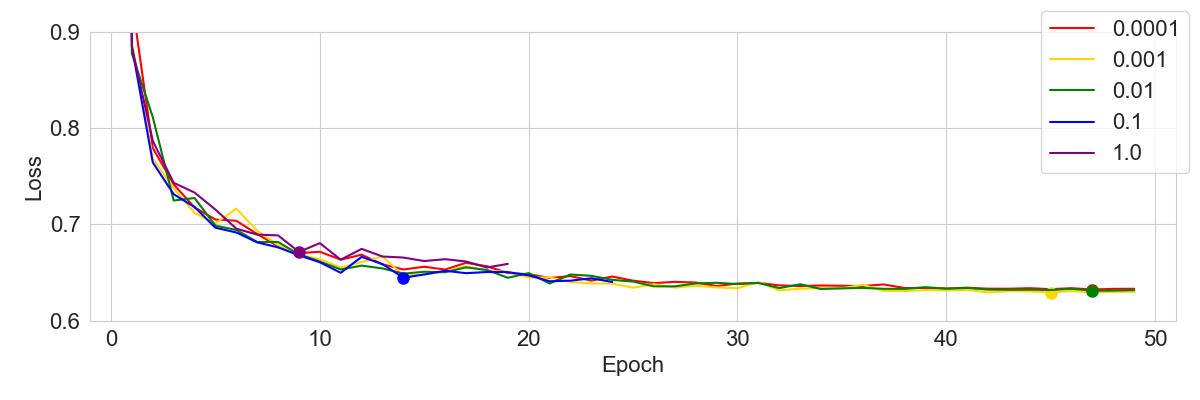
\includegraphics[height=55mm]{./figure/sec4/learning_curve/impact_of_loss_weights_across_methods/0/mel_loss.png}
        \caption{メルスペクトログラムのMAE Loss(式~\eqref{sec4:eq:loss}の$L_{mel}$)}
        \label{sec4:fig:learning_curve_method_1_val_mel_loss}
    \end{subfigure}
    \begin{subfigure}{\linewidth}
        \centering
        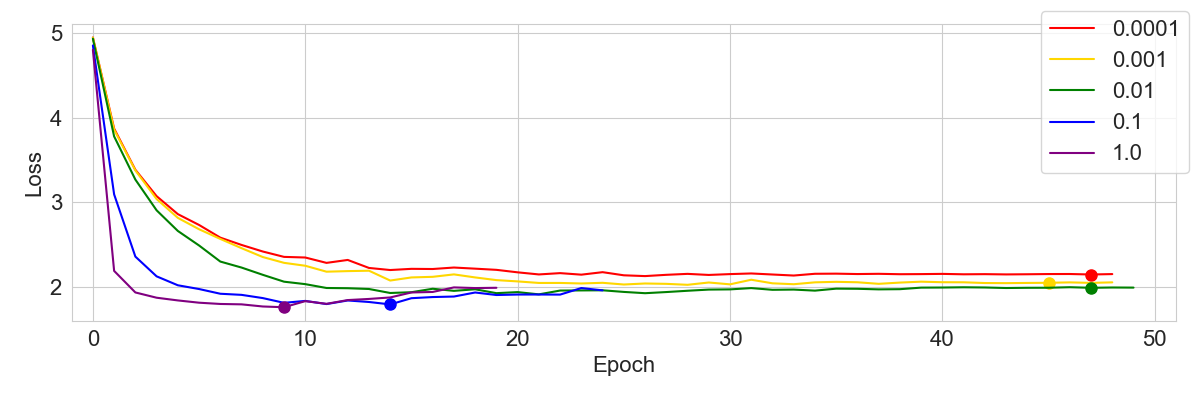
\includegraphics[height=55mm]{./figure/sec4/learning_curve/impact_of_loss_weights_across_methods/0/ssl_feature_cluster_loss.png}
        \caption{HuBERT離散特徴量のCross Entropy Loss(式~\eqref{sec4:eq:loss}の$L_{ssl^{d}}$)}
        \label{sec4:fig:learning_curve_method_1_val_ssl_feature_cluster_loss}
    \end{subfigure}
    \begin{subfigure}{\linewidth}
        \centering
        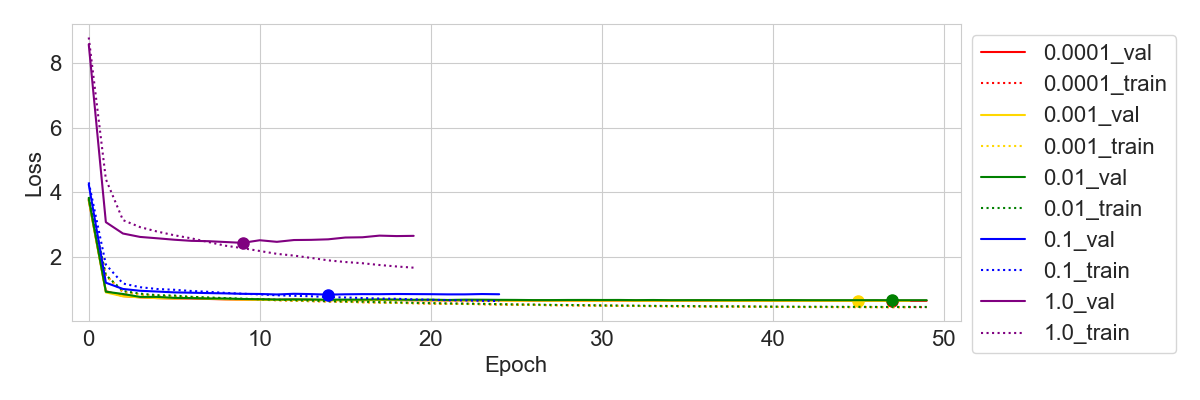
\includegraphics[height=55mm]{./figure/sec4/learning_curve/impact_of_loss_weights_across_methods/0/total_loss.png}
        \caption{損失の合計値(式~\eqref{sec4:eq:loss}の$L$)}
        \label{sec4:fig:learning_curve_method_1_val_total_loss}
    \end{subfigure}
    \caption{手法1における学習曲線}
    \label{sec4:fig:learning_curve_method_1_val_losses}
\end{figure}

\begin{figure}[bt]
    \centering
    \begin{subfigure}{\linewidth}
        \centering
        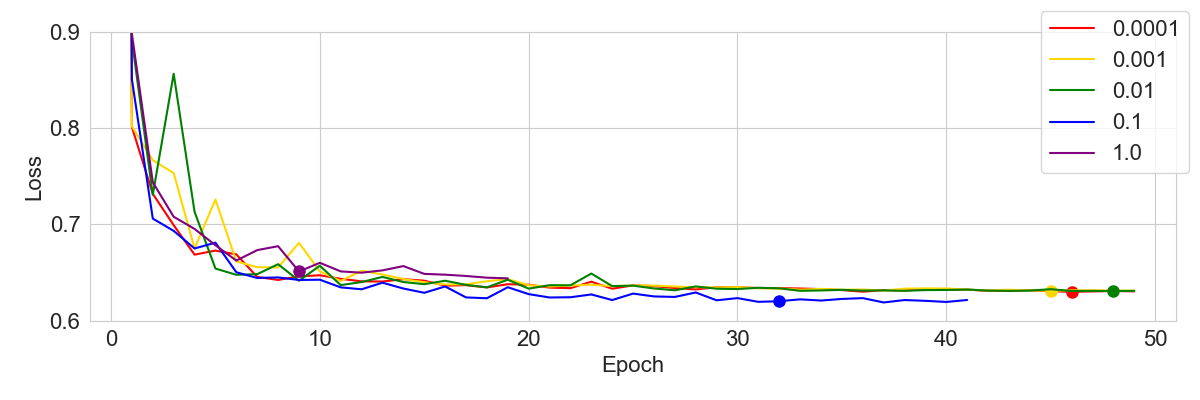
\includegraphics[height=55mm]{./figure/sec4/learning_curve/impact_of_loss_weights_across_methods/2/mel_loss.png}
        \caption{メルスペクトログラムのMAE Loss(式~\eqref{sec4:eq:loss}の$L_{mel}$)}
        \label{sec4:fig:learning_curve_method_2_val_mel_loss}
    \end{subfigure}
    \begin{subfigure}{\linewidth}
        \centering
        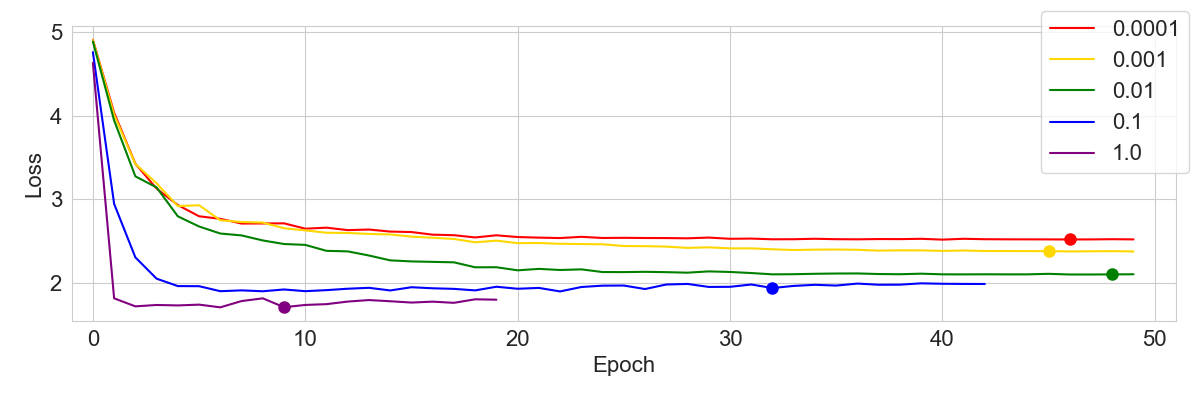
\includegraphics[height=55mm]{./figure/sec4/learning_curve/impact_of_loss_weights_across_methods/2/ssl_feature_cluster_loss.png}
        \caption{HuBERT離散特徴量のCross Entropy Loss(式~\eqref{sec4:eq:loss}の$L_{ssl^{d}}$)}
        \label{sec4:fig:learning_curve_method_2_val_ssl_feature_cluster_loss}
    \end{subfigure}
    \begin{subfigure}{\linewidth}
        \centering
        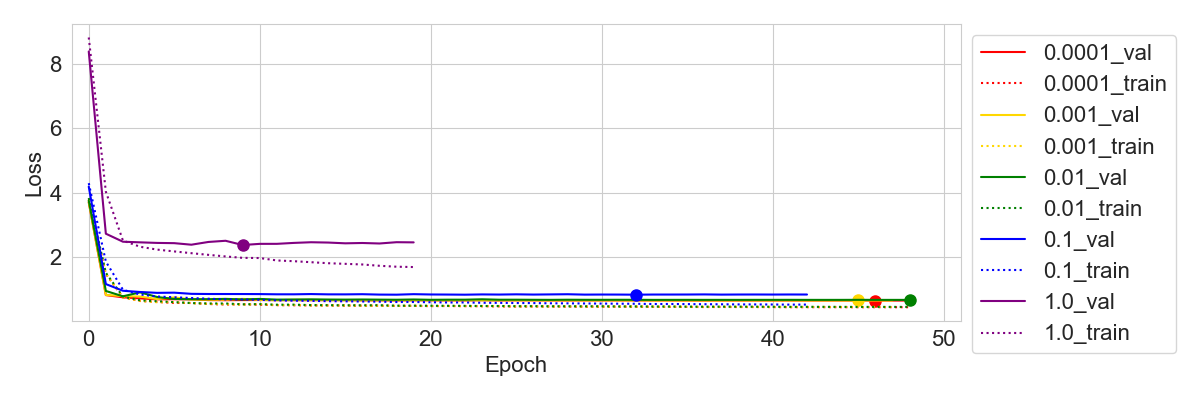
\includegraphics[height=55mm]{./figure/sec4/learning_curve/impact_of_loss_weights_across_methods/2/total_loss.png}
        \caption{損失の合計値(式~\eqref{sec4:eq:loss}の$L$)}
        \label{sec4:fig:learning_curve_method_2_val_total_loss}
    \end{subfigure}
    \caption{手法2における学習曲線}
    \label{sec4:fig:learning_curve_method_2_val_losses}
\end{figure}

\begin{figure}[bt]
    \centering
    \begin{subfigure}{\linewidth}
        \centering
        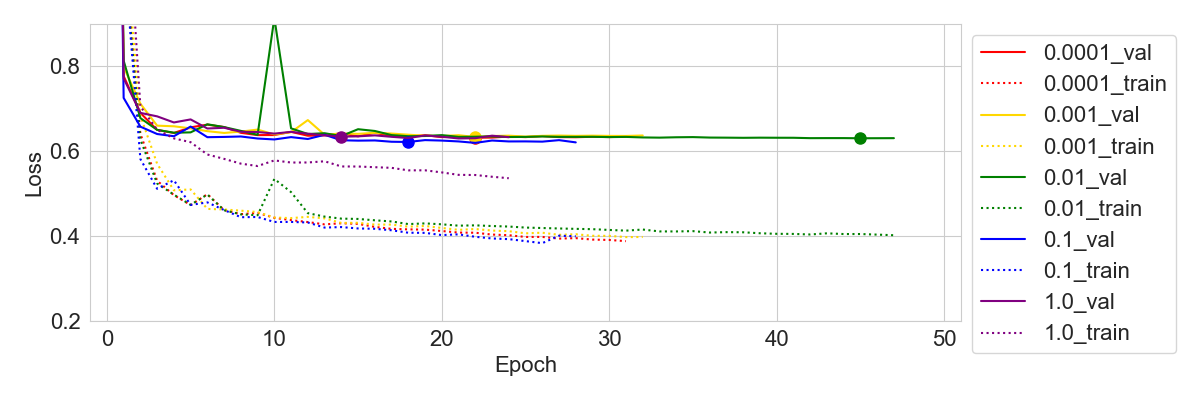
\includegraphics[height=55mm]{./figure/sec4/learning_curve/impact_of_loss_weights_across_methods/3/mel_loss.png}
        \caption{メルスペクトログラムのMAE Loss(式~\eqref{sec4:eq:loss}の$L_{mel}$)}
        \label{sec4:fig:learning_curve_method_3_val_mel_loss}
    \end{subfigure}
    \begin{subfigure}{\linewidth}
        \centering
        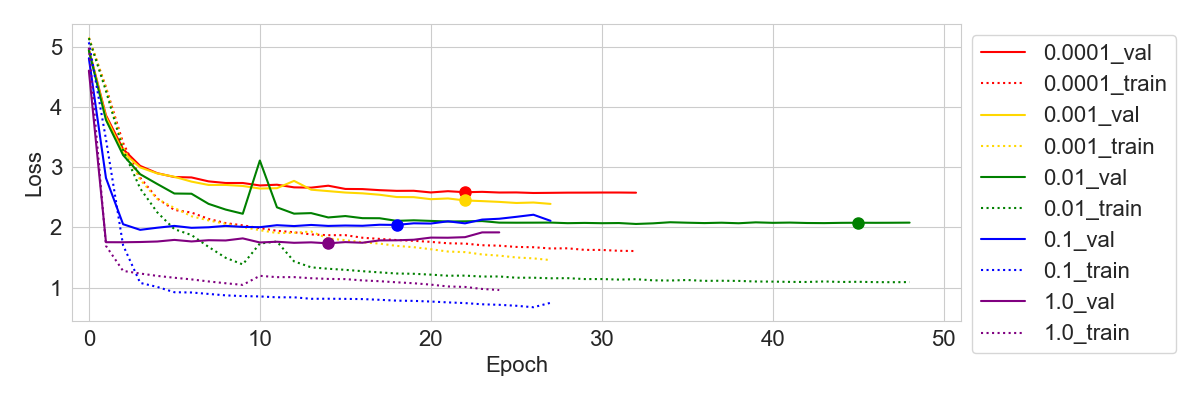
\includegraphics[height=55mm]{./figure/sec4/learning_curve/impact_of_loss_weights_across_methods/3/ssl_feature_cluster_loss.png}
        \caption{HuBERT離散特徴量のCross Entropy Loss(式~\eqref{sec4:eq:loss}の$L_{ssl^{d}}$)}
        \label{sec4:fig:learning_curve_method_3_val_ssl_feature_cluster_loss}
    \end{subfigure}
    \begin{subfigure}{\linewidth}
        \centering
        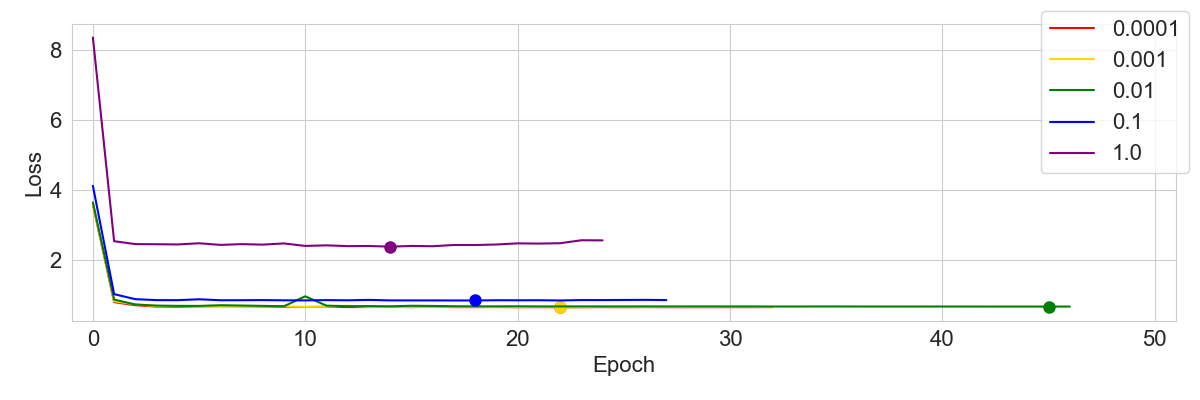
\includegraphics[height=55mm]{./figure/sec4/learning_curve/impact_of_loss_weights_across_methods/3/total_loss.png}
        \caption{損失の合計値(式~\eqref{sec4:eq:loss}の$L$)}
        \label{sec4:fig:learning_curve_method_3_val_total_loss}
    \end{subfigure}
    \caption{手法3における学習曲線}
    \label{sec4:fig:learning_curve_method_3_val_losses}
\end{figure}

\begin{figure}[bt]
    \centering
    \begin{subfigure}{\linewidth}
        \centering
        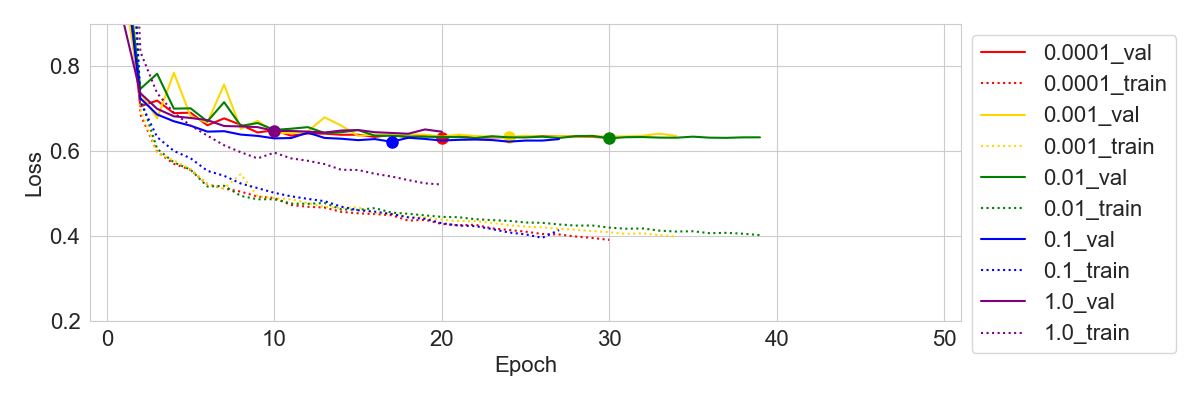
\includegraphics[height=55mm]{./figure/sec4/learning_curve/impact_of_loss_weights_across_methods/4/mel_loss.png}
        \caption{メルスペクトログラムのMAE Loss(式~\eqref{sec4:eq:loss}の$L_{mel}$)}
        \label{sec4:fig:learning_curve_method_4_val_mel_loss}
    \end{subfigure}
    \begin{subfigure}{\linewidth}
        \centering
        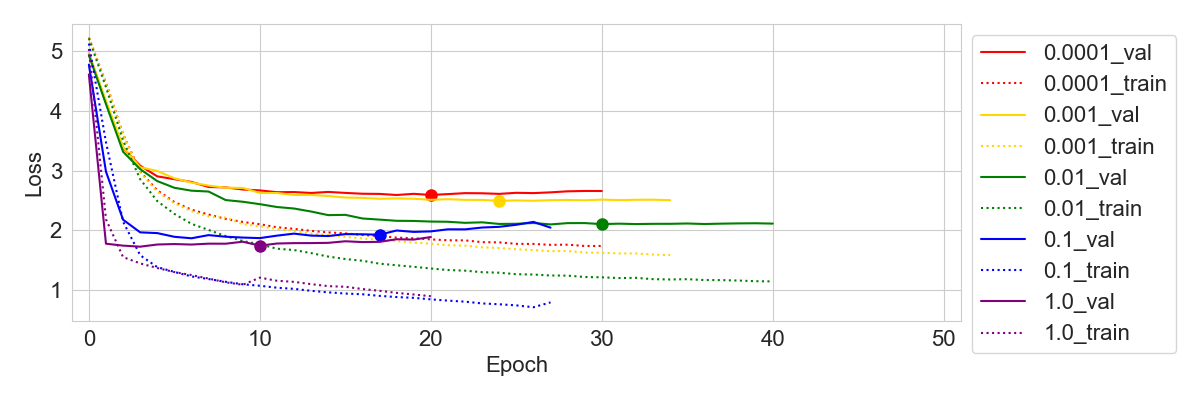
\includegraphics[height=55mm]{./figure/sec4/learning_curve/impact_of_loss_weights_across_methods/4/ssl_feature_cluster_loss.png}
        \caption{HuBERT離散特徴量のCross Entropy Loss(式~\eqref{sec4:eq:loss}の$L_{ssl^{d}}$)}
        \label{sec4:fig:learning_curve_method_4_val_ssl_feature_cluster_loss}
    \end{subfigure}
    \begin{subfigure}{\linewidth}
        \centering
        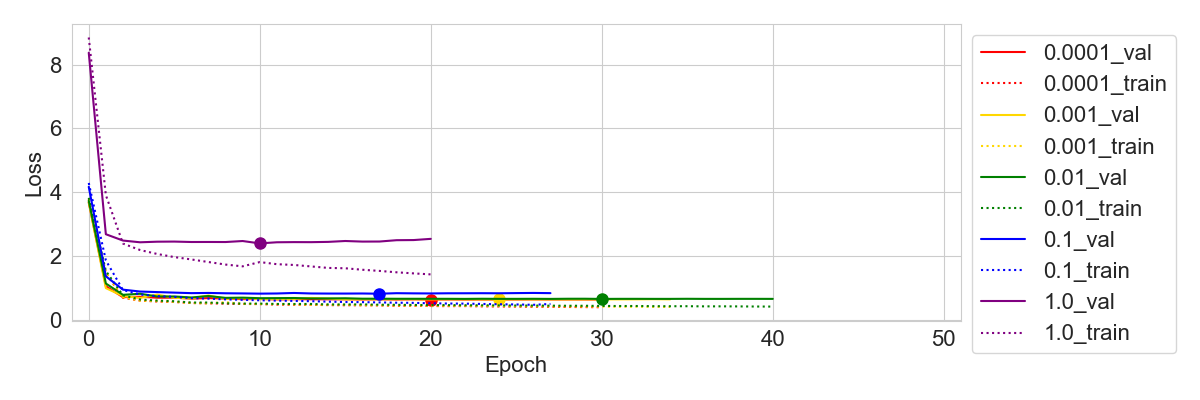
\includegraphics[height=55mm]{./figure/sec4/learning_curve/impact_of_loss_weights_across_methods/4/total_loss.png}
        \caption{損失の合計値(式~\eqref{sec4:eq:loss}の$L$)}
        \label{sec4:fig:learning_curve_method_4_val_total_loss}
    \end{subfigure}
    \caption{手法4における学習曲線}
    \label{sec4:fig:learning_curve_method_4_val_losses}
\end{figure}

\begin{figure}[bt]
    \centering
    \begin{subfigure}{\linewidth}
        \centering
        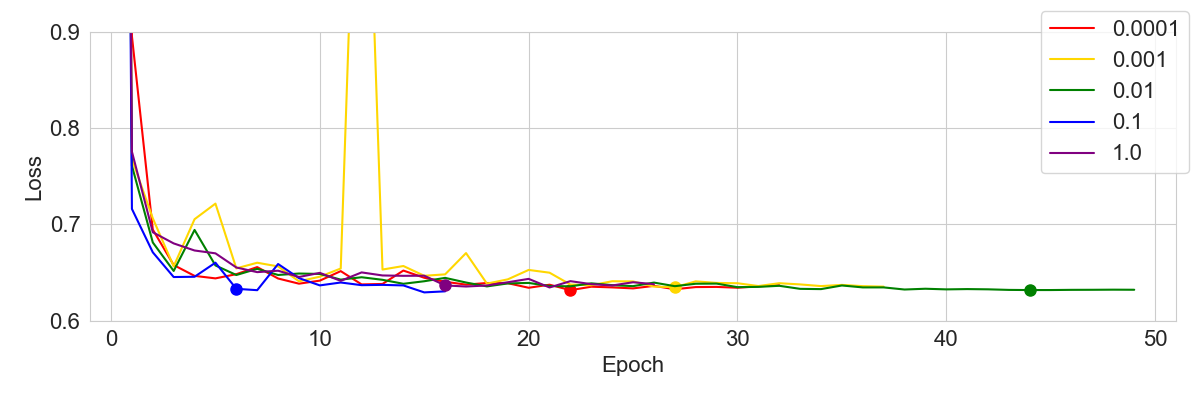
\includegraphics[height=55mm]{./figure/sec4/learning_curve/impact_of_loss_weights_across_methods/5/mel_loss.png}
        \caption{メルスペクトログラムのMAE Loss(式~\eqref{sec4:eq:loss}の$L_{mel}$)}
        \label{sec4:fig:learning_curve_method_5_val_mel_loss}
    \end{subfigure}
    \begin{subfigure}{\linewidth}
        \centering
        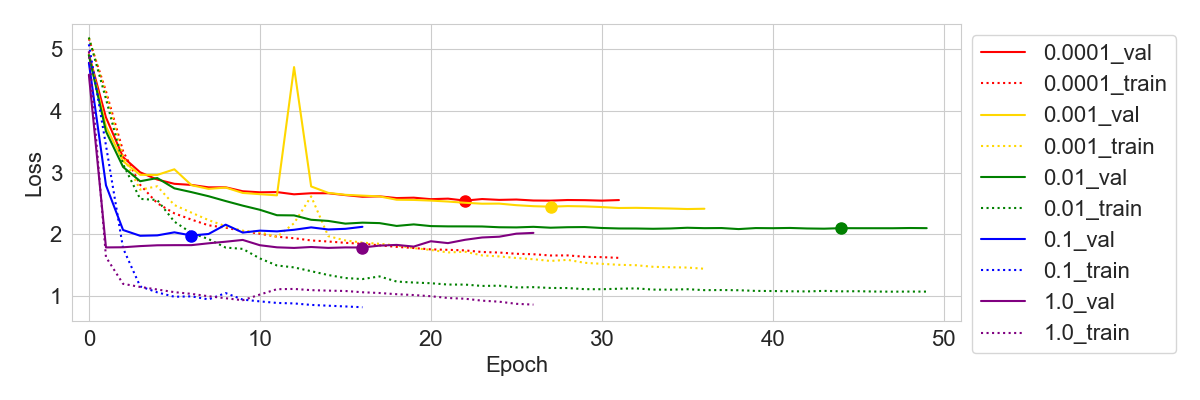
\includegraphics[height=55mm]{./figure/sec4/learning_curve/impact_of_loss_weights_across_methods/5/ssl_feature_cluster_loss.png}
        \caption{HuBERT離散特徴量のCross Entropy Loss(式~\eqref{sec4:eq:loss}の$L_{ssl^{d}}$)}
        \label{sec4:fig:learning_curve_method_5_val_ssl_feature_cluster_loss}
    \end{subfigure}
    \begin{subfigure}{\linewidth}
        \centering
        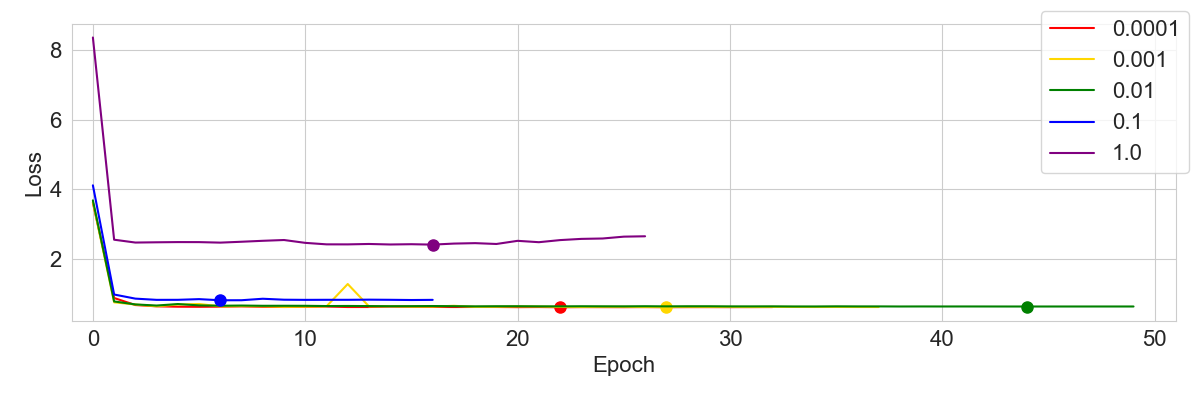
\includegraphics[height=55mm]{./figure/sec4/learning_curve/impact_of_loss_weights_across_methods/5/total_loss.png}
        \caption{損失の合計値(式~\eqref{sec4:eq:loss}の$L$)}
        \label{sec4:fig:learning_curve_method_5_val_total_loss}
    \end{subfigure}
    \caption{手法5における学習曲線}
    \label{sec4:fig:learning_curve_method_5_val_losses}
\end{figure}

\begin{table*}[bt]
    \centering
    \caption{最適なチューニングをした場合における手法ごとの比較}
    \label{sec4:tab:obj_method_comp}
    \begin{center}
        \renewcommand{\arraystretch}{1.0} % 行の高さ調整
        \setlength{\tabcolsep}{8pt}      % 列の幅調整
        \scalebox{1.0}{
            \begin{tabular}{|c|l|rr|}
                \hline
                \multicolumn{1}{|c|}{手法} & \multicolumn{1}{c|}{詳細}     & \multicolumn{1}{c}{WER [\%]} & \multicolumn{1}{c|}{話者類似度} \\
                \hline
                1                        & ベースライン                      & 55.3                         & 0.841                      \\
                2                        & ランダム初期化Transformer          & 46.2                         & 0.844                      \\
                3                        & ランダム初期化Transformer + アンサンブル & \underline{45.8}             & \underline{0.851}          \\
                4                        & 事前学習ありTransformer           & 47.4                         & 0.827                      \\
                5                        & 事前学習ありTransformer + アンサンブル  & 47.4                         & 0.810                      \\
                \hline
                6                        & 分析合成                        & 4.8                          & 0.944                      \\
                7                        & 原音声                         & 4.5                          & 1.000                      \\
                \hline
            \end{tabular}
        }
    \end{center}
\end{table*}

\begin{figure}[bt]
    \centering
    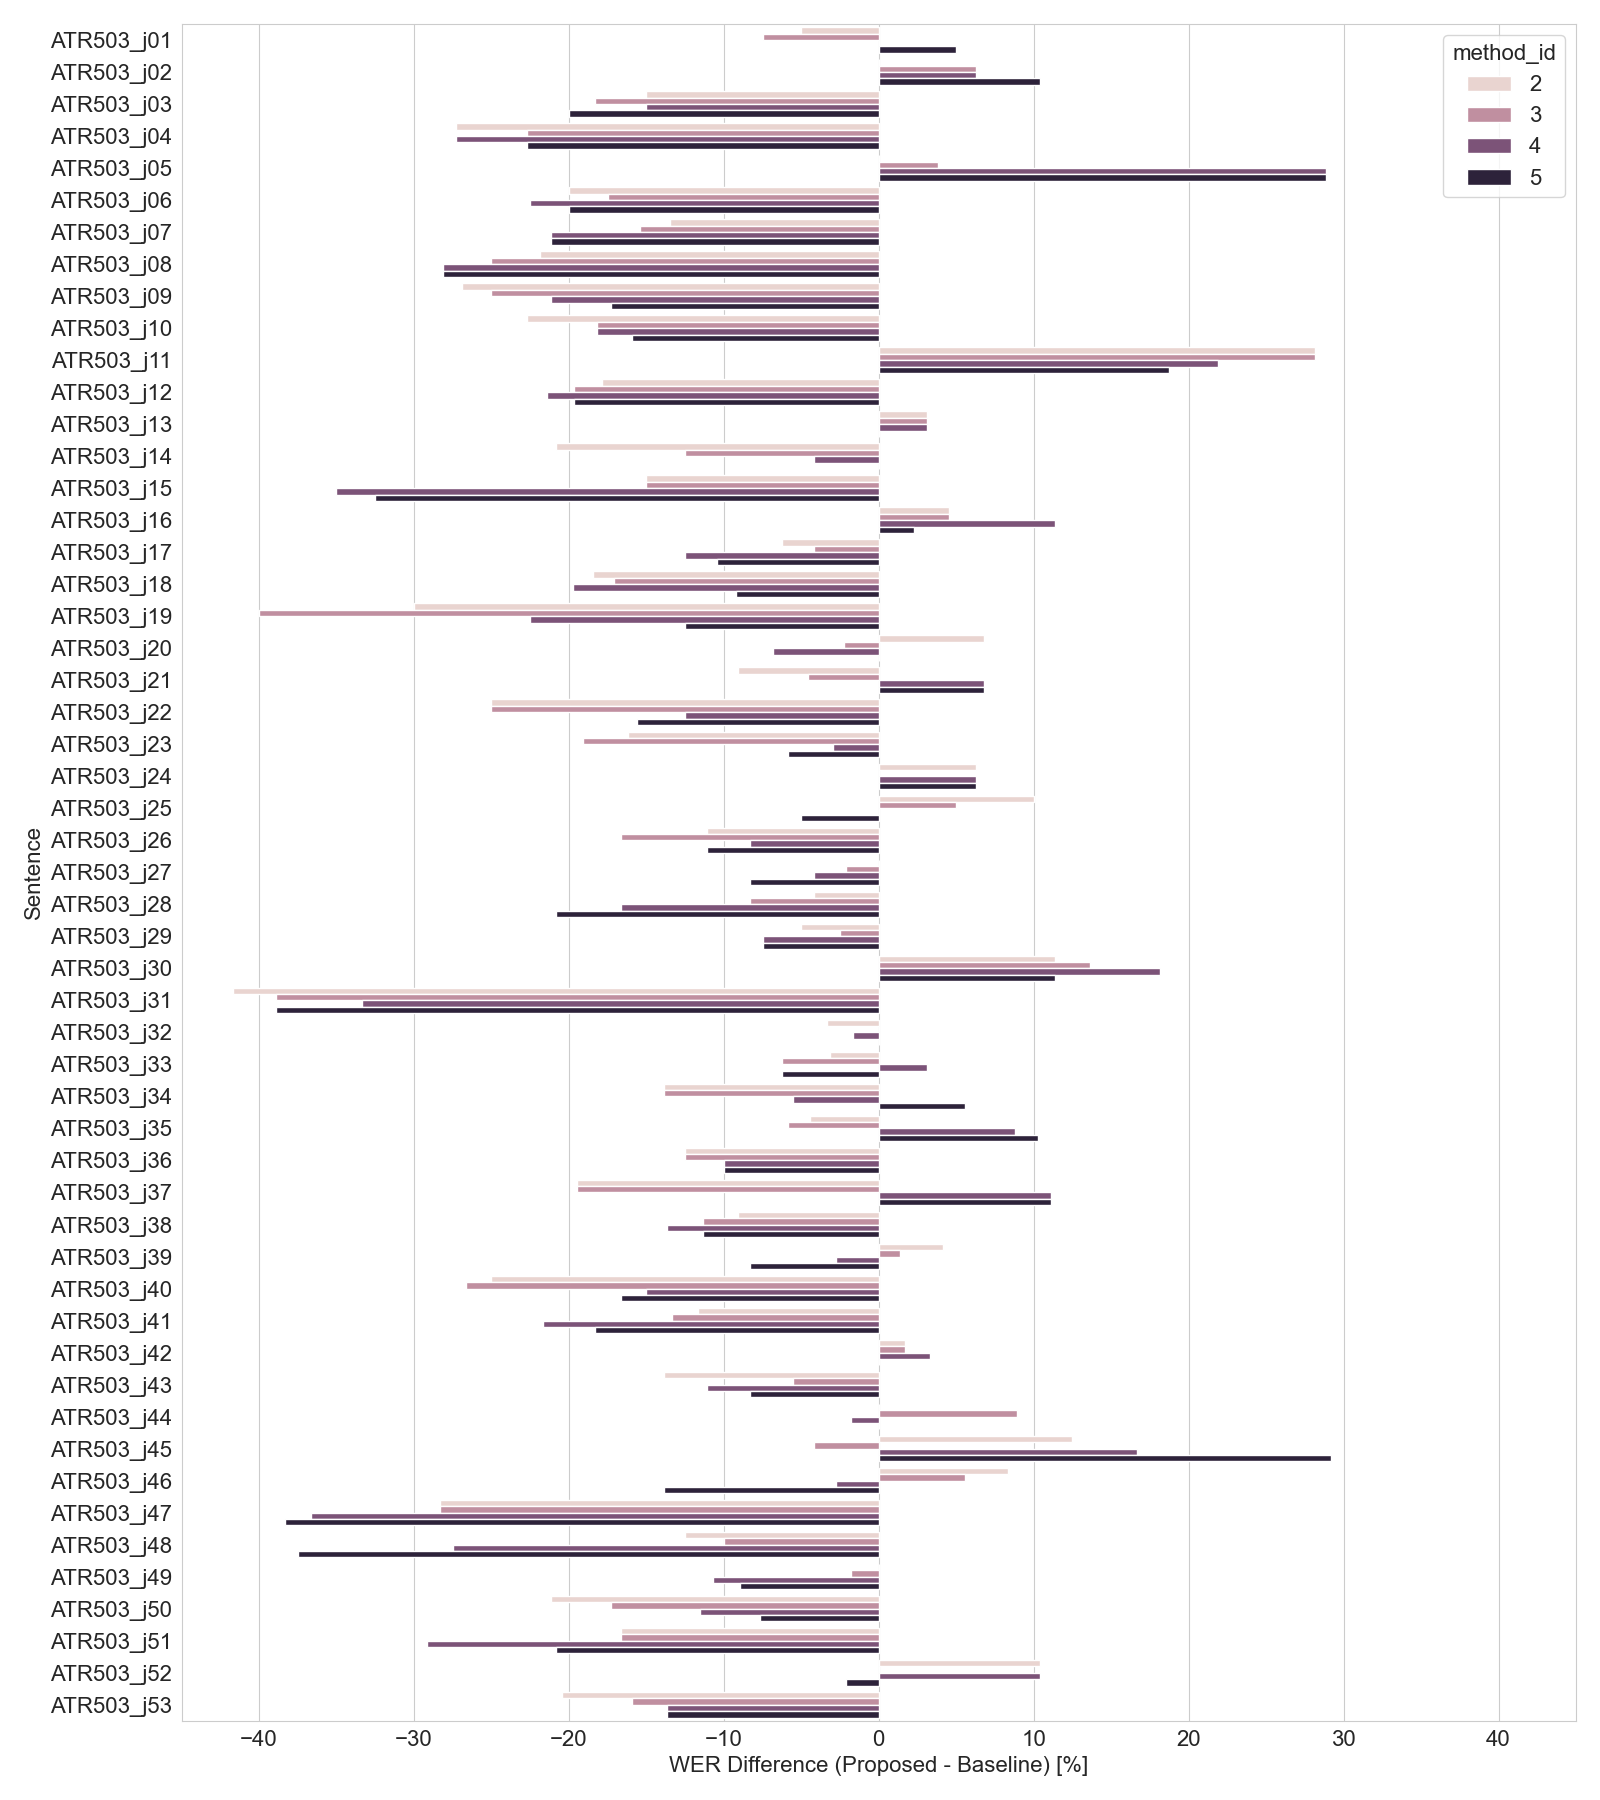
\includegraphics[height=190mm]{./figure/sec4/obj_metrics/wer_sample_wise_comparison.png}
    \caption{テストデータにおける発話文章ごとのWERの比較}
    \label{sec4:fig:wer_sample_wise_comparison}
\end{figure}

\begin{figure}[bt]
    \centering
    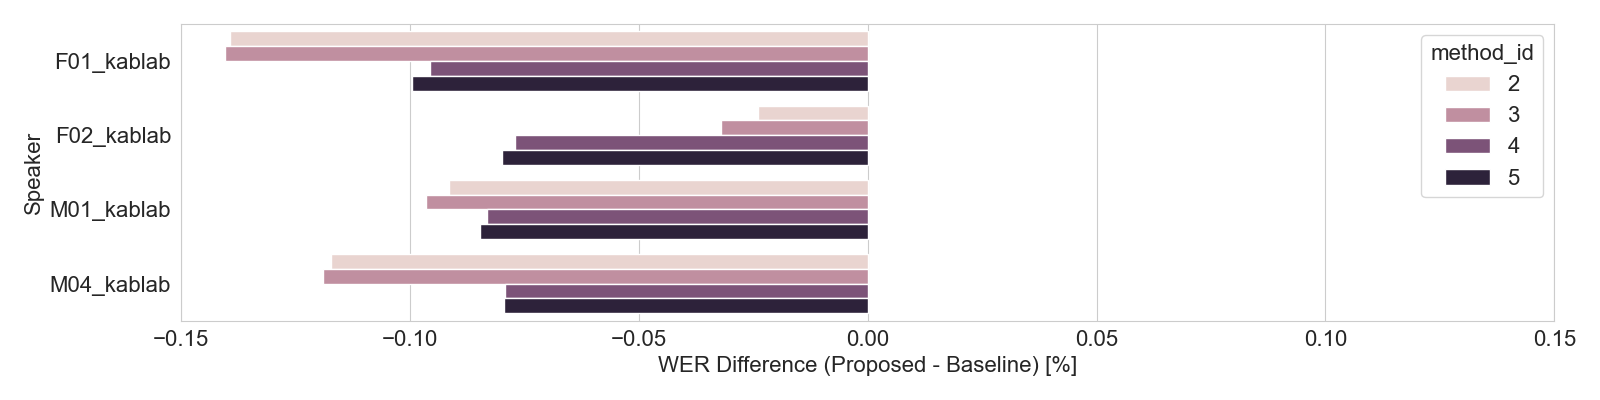
\includegraphics[height=40mm]{./figure/sec4/obj_metrics/wer_speaker_wise_comparison.png}
    \caption{テストデータにおける話者ごとのWERの比較}
    \label{sec4:fig:wer_speaker_wise_comparison}
\end{figure}

\begin{figure}[bt]
    \centering
    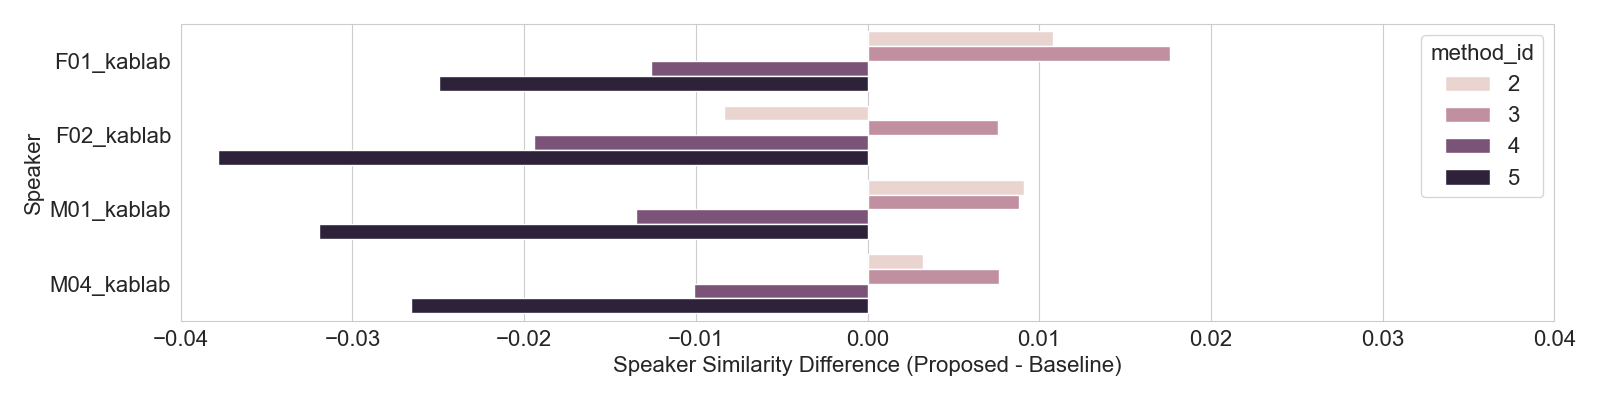
\includegraphics[height=40mm]{./figure/sec4/obj_metrics/spk_sim_speaker_wise_comparison.png}
    \caption{テストデータにおける話者ごとの話者類似度の比較}
    \label{sec4:fig:spk_sim_speaker_wise_comparison}
\end{figure}

\clearpage

\subsubsection{主観評価}

\clearpage

\subsection{まとめ}

\clearpage

% \section{音声SSLモデルを活用した動画音声合成の検討}
% \label{音声SSLモデルを活用した動画音声合成の検討}
% 本章では、音声SSLモデルであるHuBERTを利用した動画音声合成モデルを提案する。実験では比較手法として先行研究\cite{choi2023intelligible}のアプローチを含みつつ、モデルの予測対象についても複数検討した。

% \subsection{音声合成法}
% 提案手法の構築手順は二段階に分かれる。ネットワークの概要を図~\ref{sec4:fig:network}に示す。まず、動画を入力として、メルスペクトログラムとHuBERT中間特徴量を推定するネットワークを学習する(図~\ref{sec4:fig:network}-A)。HuBERT中間特徴量は、HuBERTにおける畳み込み層出力のことを指す。ここでは、AVHuBERTを動画からの特徴抽出に利用した。AVHuBERTにはパラメータ数が1億程度のBaseモデルと、3億程度のLargeモデルが存在するが、本研究では計算機のメモリの都合上、Baseモデルのみを検討した。AVHuBERTへの音声特徴量は、先行研究と同様に0で埋めた特徴量を入力した。これによって動画のみを入力した下流タスクへのFineTuningが可能となる。この出力に対して、手法~\cite{wan2018generalized}によって音声波形から得られる話者Embeddingをチャンネル方向に結合する。その後、畳み込み層からなるデコーダを通すことによって、話者Embeddingを新たに結合した特徴量に対する変換を施した。デコーダは残差結合を利用したブロック単位で構成され、各ブロックに2層の畳み込み層を設けた。畳み込み層のカーネルサイズは3とし、2ブロック積み重ねた。最後に、全結合層に通すことによって所望の出力を得る。一度チャンネルサイズ \texttimes 出力特徴量のフレーム数まで次元を拡張し、その後reshapeすることによって所望の次元、フレーム数となった最終出力を得た。

% 次に、一段階目に学習されたネットワークの重みを固定した状態でHuBERT中間特徴量を推定し、それを入力としてHuBERTのTransformer層の学習を行う(図~\ref{sec4:fig:network}-B)。ここでは、原音声から計算されたHuBERT出力特徴量(音声SSL特徴量)を推定対象とする。HuBERTの自己教師あり学習においてマスクが適用されるのは畳み込み層出力であるため、その後のTransformer層を本研究のタスクにFine Tuningすることにより、推定残差の軽減を狙った。予測対象として以下三種類を検討した。
% \begin{enumerate}
%     \item 音声SSL特徴量の連続値自体をそのまま予測対象とする場合(音声SSL連続特徴量)
%     \item 音声SSL特徴量をk-means法によるクラスタリングで離散化し、そのクラスタを予測対象とする場合(音声SSL離散特徴量)
%     \item 上記二つのマルチタスク学習の場合
% \end{enumerate}

% 以上のモデルを組み合わせることで、動画から音響特徴量の推定が可能になる。具体的には、一段階目に得られるモデルに動画を入力することでメルスペクトログラムとHuBERT中間特徴量を推定し、そのうちHuBERT中間特徴量をFineTuningされたHuBERTのTransformer層に入力することで、音声SSL特徴量が得られる。その後、先行研究~\cite{choi2023intelligible}に基づくMulti-input Vocoderを用い、メルスペクトログラムと音声SSL特徴量を入力として音声波形に変換することで、最終的な合成音声を得たMulti-input VocoderはHifi-gan~\cite{kong2020hifi}をベースとしたモデルである。本研究では動画から予測される音響特徴量が複数パターン存在するため、そのパターンごとに別個でボコーダを学習した。

% \begin{figure}[bt]
%     \centering
%     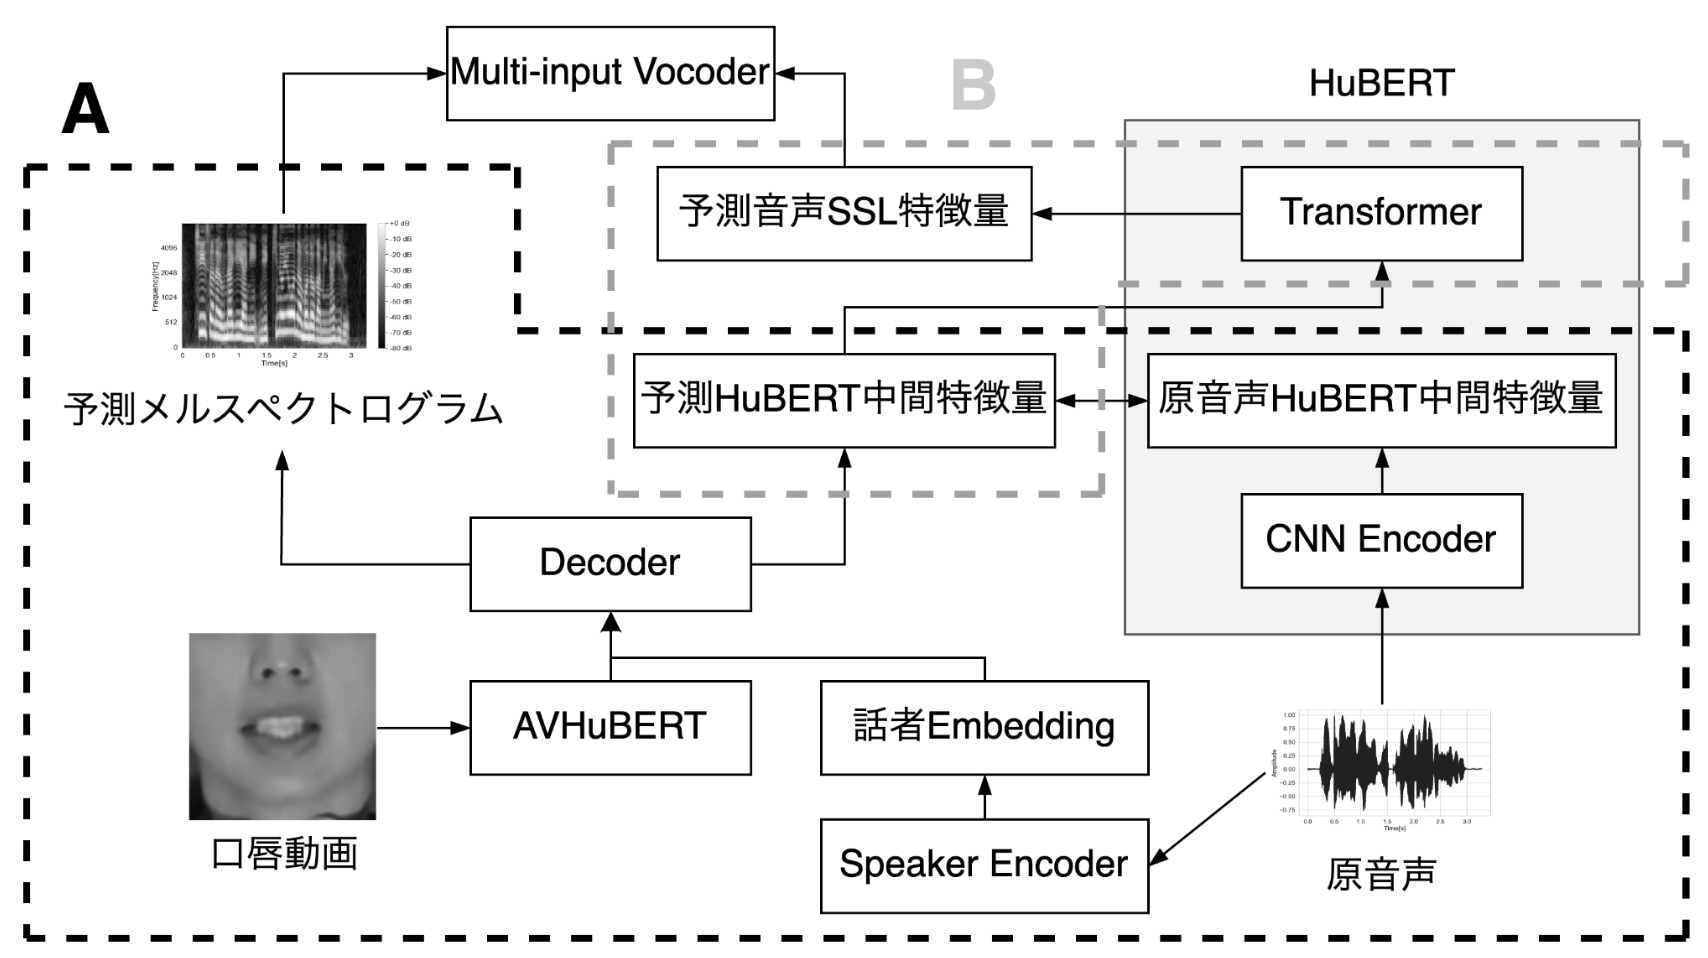
\includegraphics[height=90mm]{./figure/sec4/network.png}
%     \caption{ネットワークの概略図}
%     \label{sec4:fig:network}
% \end{figure}

% \subsection{実験方法}
% \subsubsection{利用したデータセット}
% 動画音声データセットには、男女二人ずつから収録した合計4人分のデータセット~\cite{taguchi,esaki}を用いた。これはATR音素バランス文~\cite{atr}から構成され、全話者共通でAからHセットを学習データ、Iセットを検証データ、Jセットをテストデータとして利用した。各分割ごとの文章数を表~\ref{sec4:tab:dataset_info}に示す。

% Multi-input Vocoderの学習に利用する音声データセットには、Hi-Fi-Captain(日本語話者二名分)~\cite{okamoto2023hi}とJVS(parallel100とnonpara30)~\cite{takamichi2019jvs}を利用した。ボコーダの学習時にはサンプル全体から1秒分をランダムにサンプリングして用いるのだが、元データには話し声のない無音区間が一定存在しており、これはボコーダの学習に望ましくない。これに対して、無音区間のトリミング(-40 dBFS未満かつ500 ms継続する区間を100 msまでカット)を適用した。Hi-Fi-Captainはtrain-parallelおよびtrain-non-parallelを学習データ、valを検証データ、evalをテストデータとして分割した。各分割ごとの文章数を表~\ref{sec4:tab:dataset_info}に示す。JVSには話者に対して1から100まで番号が割り振られており、本実験では1から80番の話者を学習データ、81番から90番の話者を検証データ、91番から100番までの話者をテストデータとした。各分割ごとの文章数を表~\ref{sec4:tab:dataset_info}に示す。

% \begin{table*}[bt]
%     \centering
%     \caption{利用したデータセットの文章数}
%     \label{sec4:tab:dataset_info}
%     \begin{center}
%         \renewcommand{\arraystretch}{0.9} % 行の高さ調整
%         \setlength{\tabcolsep}{8pt}      % 列の幅調整
%         \scalebox{1.0}{
%             \begin{tabular}{|l|r|r|r|}
%                 \hline
%                               & \multicolumn{1}{c|}{学習} & \multicolumn{1}{c|}{検証} & \multicolumn{1}{c|}{テスト} \\
%                 \hline
%                 動画音声データセット    & 1600                    & 200                     & 212                      \\
%                 Hi-Fi-Captain &                         &                         &                          \\
%                 JVS           &                         &                         &                          \\
%                 \hline
%             \end{tabular}
%         }
%     \end{center}
% \end{table*}

% \subsubsection{データの前処理}
% 動画データは60 FPSで収録されたものをffmpegにより25 FPSに変換して用いた。その後、手法~\cite{bulat2017far}により動画に対してランドマーク検出を適用した。このランドマークを利用することで口元のみを切り取り、画像サイズを(96, 96)にリサイズした上で、グレースケールに変換した。加えて、画像に対する正規化および標準化を適用した。学習時は、ランダムクロップ、左右反転、Time Masking(一時停止)をデータ拡張として適用した。ランダムクロップは、(96, 96)で与えられる画像から(88, 88)をランダムに切り取る処理である。検証およびテスト時は、必ず画像中央を切り取るよう実装した。左右反転はランダムクロップ後に適用しており、50\%の確率で左右が反転されるよう実装した。Time Maskingは、連続する画像の時間平均値を利用することによって、一時停止させるような効果を与えるデータ拡張手法である。動画1秒あたり0から0.5秒の間でランダムに停止区間を定め、その区間における動画の時間方向平均値を計算し、区間内のすべてのフレームをこの平均値で置換した。

% 音声データは48 kHzで収録されたものを16 kHzにダウンサンプリングして用いた。それから、窓長25 msのハニング窓を用いて、シフト幅10 msでSTFTを適用することでフレームレート100 Hzのスペクトログラムに変換した。さらに、振幅スペクトログラムに対して80次のメルフィルタバンクを適用し、80次のメルスペクトログラムを得た上で対数スケールに変換した。話者Embeddingの取得には事前学習済みモデル~\cite{wan2018generalized}を利用し、学習データから100個ランダムサンプリングして計算した平均値を利用した。

% HuBERTは、HuggingFaceに公開されているReazonSpeechというデータセットによって学習されたモデル~\cite{rinna-japanese-hubert-base,sawada2024release}を利用した。ReazonSpeechは約19000時間の日本語音声からなるデータセットであり、日本語音声のコンテキストを大量のデータから学習したモデルになっていることが予想される。本研究のアプローチでは、日本語音声に関する事前知識を豊富に有するモデルが適していると考え、このモデルを選択した。検討した予測対象の一つである音声SSL離散特徴量は、k-means法によるクラスタリング(クラスタ数200)によって得た。クラスタ数は、今回比較する先行研究~\cite{choi2023intelligible}に基づいている。このモデルの学習にはHi-Fi-Captainを利用しており、男性女性それぞれ学習データ全体から50\%をランダムサンプリングして用いた。

% \subsubsection{学習方法}
% 第一段階であるAVHuBERTをベースとしたモデルの学習について、損失関数はメルスペクトログラムについてのMAE Lossと、HuBERT中間特徴量のMAE Lossの和とした。最適化手法にはAdamW~\cite{loshchilov2017decoupled}を利用し、$\beta_{1} = 0.9$、$\beta_{2} = 0.98$、$weight\_decay = 0.01$とした。学習率は\num{1.0e-3}から開始し、Warmup Schedulerによってその値を変化させた。バッチサイズはメモリの都合上4としたが、学習の安定のためGradient Accumulationによって各イテレーションにおける勾配を累積させ、8イテレーションに一回重みを更新するようにした。そのため、実質的にはバッチサイズ32となる。モデルに入力する動画の秒数は10秒を上限とし、それを超える場合はランダムにトリミング、それに満たない場合はゼロパディングした。勾配のノルムは3.0を上限としてクリッピングすることで、過度に大きくなることを防止した。最大エポック数は50とし、10エポック連続して検証データに対する損失が小さくならない場合には、学習を中断するようにした。また、学習終了時には検証データに対する損失が最も小さかったエポックにおけるチェックポイントを保存し、これをテストデータに対する評価に用いた。

% 第二段階であるHuBERTをベースとしたモデルの学習について、音声SSL連続特徴量に対する損失関数にはMAE Loss、音声SSL離散特徴量に対する損失関数にはCross Entropy Lossを使用した。マルチタスク学習を行う場合には、Cross Entropy Lossに対して重み係数をかけることでチューニングを行った。従って、マルチタスク学習時の損失関数は以下のように表される。
% \begin{equation}
%     L = L_{c} + \lambda * L_{d}
%     \label{sec4:eq:loss_}
% \end{equation}
% $L_{c}$はMAE Loss、$L_{d}$はCross Entropy Lossであり、$\lambda$がCross Entropy Lossにかかる重み係数を表す。本実験では$\lambda = \num{1.0e-4}$から1.0まで、10倍刻みで5段階検討した。
% 最適化手法にはAdamWを利用し、$\beta_{1} = 0.9$、$\beta_{2} = 0.98$、$weight\_decay = 0.01$とした。学習率は\num{5.0e-4}から開始し、Warmup Schedulerによってその値を変化させた。その他学習に関わるパラメータは、第一段階における値と同じである。

% Multi-input Vocoderの学習について、これは入力される音響特徴量のバリエーションに対してそれぞれ別個にモデルを構築した。全てをまとめると以下の通りである。
% \begin{enumerate}
%     \item メルスペクトログラム
%     \item メルスペクトログラム $+$ 音声SSL連続特徴量
%     \item メルスペクトログラム $+$ 音声SSL離散特徴量
%     \item メルスペクトログラム $+$ 音声SSL連続特徴量 $+$ 音声SSL離散特徴量
% \end{enumerate}
% 学習は動画音声データセットではなく、外部データであるHi-Fi-CaptainとJVSを用いた。はじめにHi-Fi-Captainのみを用いて学習させ、その後学習済みモデルをJVSによって再学習した。Hi-Fi-Captainは男女一人ずつの文章数が豊富なデータセットであるため、高品質なモデルを構築可能であった。しかし、学習できる話者数が少ない分、学習外話者に対する合成音声の品質が低かった。そのため、一人当たりの文章数は100文章程度と少ないながらも、100人分の話者からなるJVSを利用して再学習することによって、学習外話者に対する合成音声の品質を向上させた。最適化手法にはAdamWを利用し、$\beta_{1} = 0.8$、$\beta_{2} = 0.99$、$weight_decay = 0.01$とした。学習率は\num{2.0e-4}から開始し、指数関数的にその値を変化させた。バッチサイズは16とし、ここではGradient Accumulationは利用しなかった。モデルへの入力は1秒を上限とし、それを超える場合はランダムにトリミング、それに満たない場合はゼロパディングした。勾配のノルムは3.0を上限としてクリッピングすることで、過度に大きくなることを防止した。最大エポック数は30とし、ここではEarly Stoppingは適用しなかった。また、学習終了時には検証データに対する損失(メルスペクトログラムに対するL1 Loss)が最も小さかったエポックにおけるチェックポイントを保存し、これをテストデータに対する評価に用いた。

% GPUはNVIDIA RTX A4000を利用し、計算の高速化のためAutomatic Mixed Precisionを適用した。

% \subsubsection{比較手法}
% \label{比較手法}
% 比較手法は、メルスペクトログラムのみを予測対象とするベースライン、HuBERTなしのマルチタスク学習手法~\cite{choi2023intelligible}、HuBERTありのマルチタスク学習手法(提案手法)の三種類である。ただし、マルチタスク学習手法の予測対象には、以下の三種類が存在する。
% \begin{enumerate}
%     \item 音声SSL連続特徴量
%     \item 音声SSL離散特徴量
%     \item 音声SSL連続特徴量 $+$ 音声SSL離散特徴量
% \end{enumerate}
% HuBERTなしのマルチタスク学習手法、HuBERTありのマルチタスク学習手法には上記3パターンを設けたため、比較したのは計7手法となる。

% \subsubsection{客観評価}
% 合成音声の客観評価には、PESQ~\cite{rix2001perceptual}、STOI~\cite{taal2010short}、ESTOI~\cite{taal2011algorithm}、WERの4種類の客観評価指標を使用した。PESQは音声の自然性を表す指標であり、1から5の値を取る。値が高いほど良い。STOI、ESTOIはどちらも音声の明瞭性を表す指標であり、0から1の値を取る。PESQと同様に、値が高いほど良い。ここまでの三つの指標は、TorchMetricsというライブラリを用いて算出した。WERは、Whisper~\cite{radford2023robust}による音声認識の結果から算出した単語誤り率である。合成音声がより正確に認識されるほど聞き取りやすいと考えられるため、この指標は値が低いほど良い。この計算方法については、まず、Whisperによって出力されるテキストに対して、句読点を削除した上でMeCab (日本語形態素解析エンジン)を用いて分かち書きを行い、単語に分解する。その後、jiwerというライブラリを用いてWERを計算した。

% \subsubsection{主観評価}

% \begin{figure}[bt]
%     \centering
%     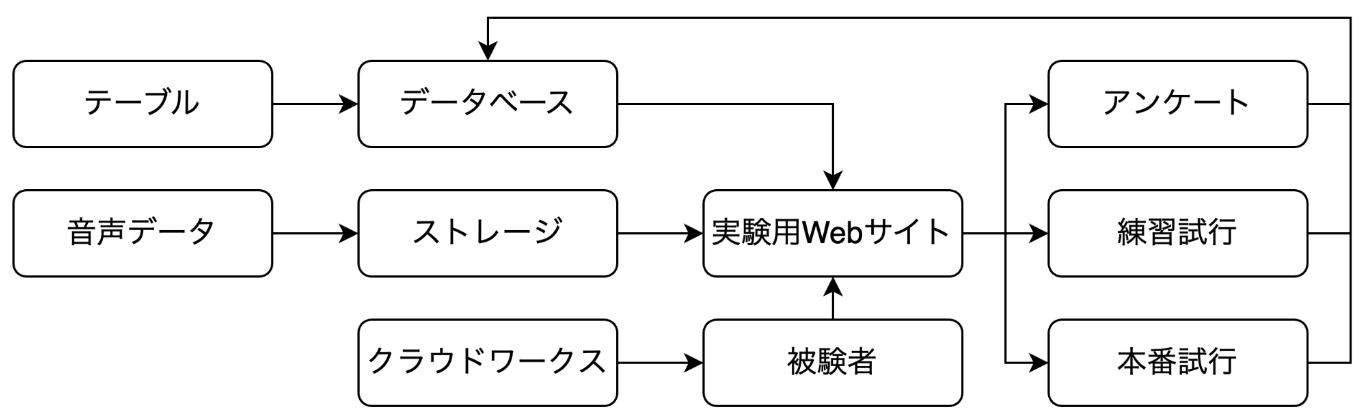
\includegraphics[height=45mm]{./figure/sec4/sbj_flow.png}
%     \caption{主観評価実験全体の流れ}
%     \label{sec4:fig:sbj_flow}
% \end{figure}

% 主観評価実験では、音声の明瞭性と自然性を実際に人に聞いていただくことで評価した。実験全体の流れを図~\ref{sec4:fig:sbj_flow}に示す。今回はクラウドワークスというクラウドソーシングサービスおよび、自作の実験用 Web サイトを利用して、オンラインで実験を実施した。実験全体の大まかな流れは以下の通りである。
% \begin{enumerate}
%     \item 音声ファイルをクラウドストレージにアップロードするとともに、実験データを管理するためのテーブルをリモートサーバーのデータベースに作成する。
%     \item クラウドワークスにて実験を公開し、被験者を募集する。
%     \item 被験者と契約後、実験用Webサイトから実験を実施していただく。結果はデータベースに格納する。
%     \item 実験終了後、データベースから評価データを取得して統計処理を実施する。
% \end{enumerate}
% 被験者の方に行っていただいた項目は以下の三つである。
% \begin{enumerate}
%     \item アンケート
%     \item 練習試行
%     \item 本番試行
% \end{enumerate}
% 一つ目のアンケートでは、被験者についての基本的な統計を取ることを目的として、性別・年齢・利用した音響機器について回答していただいた。二つ目の練習試行では、実験本番の前に実験内容を把握していただくことを目的として、練習用の実験を行っていただいた。三つ目の本番試行では、最終的に統計処理に利用する評価データを得るための、本番の実験を実施した。

% 評価項目の一つである明瞭性について、教示は以下のように行った。
% \begin{quote}
%     一つ目の評価項目である明瞭性は、\textbf{発話内容自体がどれくらい聞き取りやすかったか}を指します。

%     この評価は自然性とは異なり、発話内容の理解のしやすさに焦点を当てています。

%     各音声ごとに、下記の五段階で評価してください。
%     \begin{enumerate}
%         \item 非常に悪い
%         \item 悪い
%         \item 普通
%         \item 良い
%         \item 非常に良い
%     \end{enumerate}
% \end{quote}
% もう一つの評価項目である自然性について、教示は以下のように行った。
% \begin{quote}
%     二つ目の評価項目である自然性は、\textbf{発話内容によらず、その音声がどれくらい人間らしく自然なものに聞こえたか}を指します。

%     例えば、音質自体やイントネーションの自然さなどが評価の観点として挙げられます。

%     イントネーションなど発話内容に関連する要素も含まれますが、ここではどれくらい自然な音声であるかを評価してください。

%     発話内容の聞き取りやすさではなく、音声全体の自然さが評価の対象です。この点が明瞭性の評価と異なる部分です。

%     各音声ごとに、下記の五段階で評価してください。
%     \begin{enumerate}
%         \item 非常に悪い
%         \item 悪い
%         \item 普通
%         \item 良い
%         \item 非常に良い
%     \end{enumerate}
% \end{quote}
% 自然性は明瞭性よりも漠然としており、先行研究でも教示の仕方によって評価の傾向が変化することが報告されている\cite{dall2014rating}。そのため、自然性の教示では音質やイントネーションなど、具体的に評価していただきたい観点を示した。

% 評価対象は、~\ref{比較手法}節に示した7手法に分析合成、原音声を加えた9種類の音声である。分析合成は、原音声から計算した特徴量を入力として、Multi-input Vocoderで逆変換した合成音声である。これは、今回構築したニューラルボコーダ自体の性能を表す値であり、今回の実験における合成音声の品質上限を表すような手法である。評価文章は客観評価と同様に、ATR音素バランス文のJセット53文章を利用し、話者は学習に用いた4人分全てを用いた。すなわち、各手法ごとに212サンプル($= 53 \text{文章} \times 4 \text{話者}$)を利用した。被験者ごとの評価サンプルの割り当て方法を以下に述べ、図\ref{sec4:fig:sbj_selection}にその概要も示す。
% \begin{enumerate}
%     \item 評価に用いる53文章を9つ(評価手法の総数)のグループにランダムに分割する。各グループごとに一文章を練習試行用、それ以外の文章を本番試行用としてランダムに割り振る。
%     \item 各文章グループに一つ手法を割り当て、文章一つ一つに対して話者を一人ランダムに選択する。これにより、ある被験者一名に対してユニークな53文章からなる評価データが得られる。
% \end{enumerate}
% 上記に加えて、被験者ごとに文章グループに割り当てる手法を一つずつずらすよう実装した。この過程を表\ref{sec4:tab:sbj_selection_relation}に示す。被験者ごとに文章グループに対して割り当てる手法を1ずつずらしていくことで、文章と手法の組み合わせを効率よく網羅できるようにした\cite{king2008blizzard}。加えて、サンプル選択の過程では、すべての組み合わせについて以前に評価された回数をカウントしておくことで、サンプルの選択にランダム性を持たせつつ、すべてのサンプルが等しい回数評価されるようにした。例えば、一回選択されたサンプルと未選択のサンプルが存在する場合、一回選択されたサンプルは選択の候補から除外する。これにより、未選択のサンプルのみを対象としたランダムサンプリングを行うことで、最終的な評価回数が等しくなるよう実装した。この選択方法により、36回の実験によって$\text{(手法)} \times \text{(文章)} \times \text{(話者)}$のすべての組み合わせが一回ずつ評価されることになる。

% \begin{figure}[bt]
%     \centering
%     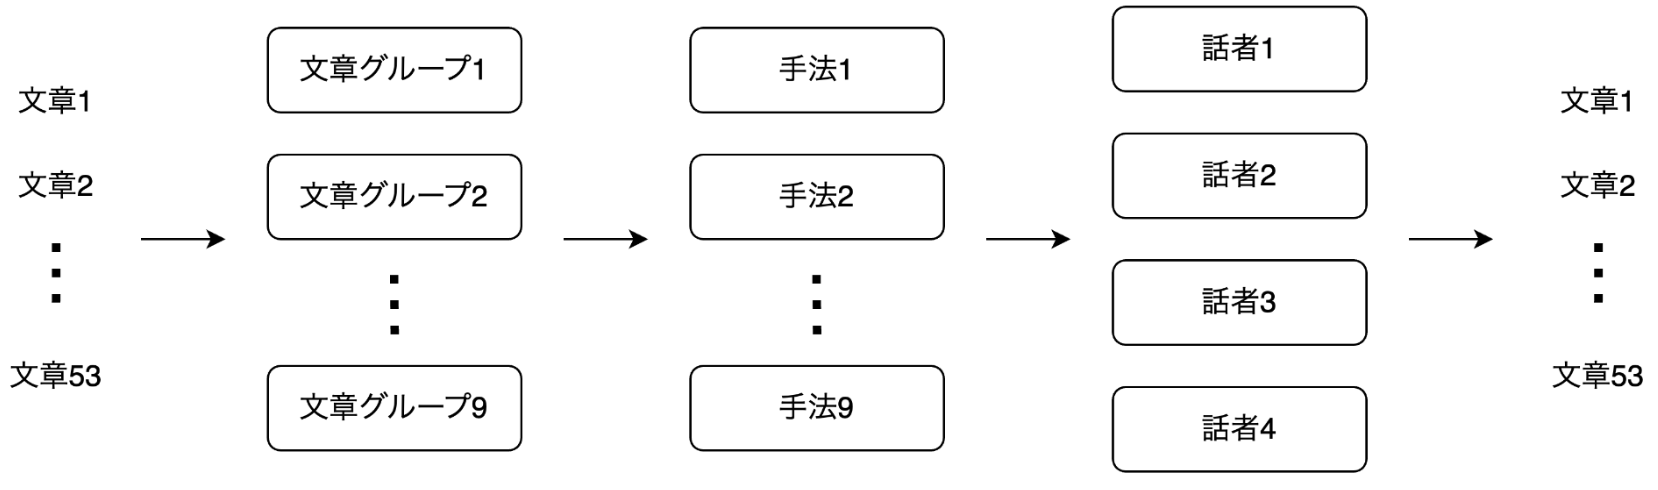
\includegraphics[height=45mm]{./figure/sec4/sbj_selection.png}
%     \caption{主観評価実験における話者ごとのサンプル選択}
%     \label{sec4:fig:sbj_selection}
% \end{figure}

% \begin{table*}[bt]
%     \centering
%     \caption{主観評価実験のサンプル選択における文章グループと手法の対応関係}
%     \label{sec4:tab:sbj_selection_relation}
%     \begin{center}
%         \renewcommand{\arraystretch}{1.0} % 行の高さ調整
%         \setlength{\tabcolsep}{8pt}      % 列の幅調整
%         \scalebox{0.9}{
%             \begin{tabular}{|c|ccccccccc|}
%                 \hline
%                 \multirow{2}{*}{}         & \multicolumn{9}{c|}{文章グループインデックス}                                 \\
%                                           & 1                                 & 2 & 3 & 4 & 5 & 6 & 7 & 8 & 9 \\
%                 \hline
%                 \multirow{9}{*}{手法インデックス} & 1                                 & 2 & 3 & 4 & 5 & 6 & 7 & 8 & 9 \\
%                                           & 2                                 & 3 & 4 & 5 & 6 & 7 & 8 & 9 & 1 \\
%                                           & 3                                 & 4 & 5 & 6 & 7 & 8 & 9 & 1 & 2 \\
%                                           & 4                                 & 5 & 6 & 7 & 8 & 9 & 1 & 2 & 3 \\
%                                           & 5                                 & 6 & 7 & 8 & 9 & 1 & 2 & 3 & 4 \\
%                                           & 6                                 & 7 & 8 & 9 & 1 & 2 & 3 & 4 & 5 \\
%                                           & 7                                 & 8 & 9 & 1 & 2 & 3 & 4 & 5 & 6 \\
%                                           & 8                                 & 9 & 1 & 2 & 3 & 4 & 5 & 6 & 7 \\
%                                           & 9                                 & 1 & 2 & 3 & 4 & 5 & 6 & 7 & 8 \\
%                 \hline
%             \end{tabular}
%         }
%     \end{center}
% \end{table*}

% 被験者数および各手法の評価回数に関して、先行研究\cite{wester2015we}では統計処理に用いる被験者数や評価回数を変数として、実験条件に対してどれほどの被験者数とサンプル数が必要そうであるかを検討している。今回はこの結果を参考に、オンラインで実験を実施するのであれば総被験者数が100人以上、各手法に対する総評価回数が200回以上となることが望ましいと判断した。前述したサンプル選択アルゴリズムにより、36回の実験によって全てのサンプルが一回ずつ評価される。これを1セットとすると、セットあたり被験者数は36人、各手法に対する評価回数は176回となる。従って、今回は3セット行うことにより、総被験者数108人、各手法に対しての総評価回数が528回となるようにした。実験一回あたり15分程度で終わると見積もって、一人当たりの報酬は250円とした。

% また、オンラインでの評価は効率よく数多くの方に評価していただけるという点でメリットがあるが、オフラインでの評価と比較して実験環境を制御することが難しく、評価の品質に不安が残る。これに対して、本実験では先行研究\cite{kirkland2023stuck}を参考に、評価サンプル中にダミー音声を混入させることで対策を講じた。ダミー音声は本研究で得られた合成音声とは無関係に、Googleのテキスト音声合成システムによって生成したサンプルである。このサンプルでは、
% \begin{quote}
%     これはダミー音声です。明瞭性は「2: 悪い」を、自然性は「1: 非常に悪い」を選択してください。
% \end{quote}
% のような音声が提示される。この時、その音声自体の明瞭性や自然性に関係なく、必ずこの音声によって指定された評価値を選択するよう教示を与えた。また、本番試行においてダミー音声で指定された評価値を誤って選んだ場合は、すべての回答を無効にし、報酬も支払うことができない旨を被験者に伝えた。実際の教示は以下のようなものである。
% \begin{quote}
%     音声サンプル内には、ダミー音声が含まれています。ダミー音声では、以下のような音声が再生されます。

%     「これはダミー音声です。明瞭性は〇〇を、自然性は〇〇を選択してください。」

%     再生した音声がダミー音声であった場合、必ずこの音声で指定された評価値を選択してください。これは、実験において適当な回答を防止するためのものです。

%     例として、下記の音声では、「これはダミー音声です。明瞭性は「2: 悪い」を、自然性は「1: 非常に悪い」を選択してください。」と指定しています。

%     (再生可能な音声サンプル)

%     この場合、明瞭性は「2: 悪い」、自然性は「1:非常に悪い」を選択します。音声自体の明瞭性や自然性を評価するわけではないため、ご注意ください。

%     特に、\textbf{本番試行においてダミー音声で指定された評価値を誤って選んだ場合は、全ての回答が無効となります。また、その場合は報酬もお支払いできません(練習試行の結果は無関係です)。}

%     誠に申し訳ありませんが、ご了承いただきますようよろしくお願い致します。
% \end{quote}

% \subsection{結果}
% \subsubsection{客観評価}
% まず、損失関数~\eqref{sec4:eq:loss}の重み係数$\lambda$を変化させた時の客観評価指標の結果を表~\ref{sec4:tab:obj_weights}に示す。最も左の列は各手法を表すIDであり、結果の説明に用いる。重み係数は離散特徴量のCross Entropy Lossについてのみ調整しているため、その対象となった3つの手法である、(2-b)、(2-c)、(3-c)を載せている。各手法ごとに0.0001から1.0まで10倍刻みで5段階検討し、各手法の客観指標ごとに最も優れた値を下線で示している。また、これ以降の実験のために、この結果から最適と考えられる重み係数の値を選択しており、それを選択フラグの列で示している。Trueが入っている行が、代表値として選択されたことを意味する。

% HuBERTなしでメルスペクトログラムと音声SSL離散特徴量を予測対象とした手法(2-b)では、特に重み係数を0.1以上とした場合に、すべての指標が顕著に悪化した。PESQについては0.0001と0.01で等しく最大値を取っている。STOI、ESTOIについては0.0001が0.01の場合よりもやや高いが、WERにおいては0.01の方が4.2\%低い。STOI、ESTOI、WERはすべて音声の明瞭性に関する指標であるため、これらが一致した傾向を示していないことから判断が難しいところではあるが、今回はWERの差が大きいことと、いずれにせよSTOI、ESTOIは比較的良好な値を示していることに着目し、0.01を代表値として選択した。HuBERTなしでメルスペクトログラムと音声SSL連続特徴量、離散特徴量を予測対象とした手法(2-c)では、重み係数0.0001の場合にPESQ、STOI、ESTOIが最大値を示した。WERについては0.1の場合に最低値である52.6\%が得られているが、その他3つの指標全てで0.0001の場合に劣っている。そのため、ここでは0.0001を代表値として選択した。HuBERTありでメルスペクトログラムと音声SSL連続特徴量、離散特徴量を予測対象とした手法(3-c)では、重み係数0.0001から0.01までの3段階は概ね同様な値を示し、それよりも重みを大きくすることですべての指標が改善する結果となった。0.1と1.0の場合はほとんど同等であるが、0.1の場合の方がPESQがやや優れていることから、こちらを代表値として選択した。

% 次に、今回構築した全手法の客観評価指標を表~\ref{sec:tab:obj_all}に示す。分析合成は、原音声から計算した特徴量を入力として、Multi-input Vocoderで逆変換した合成音声である。表~\ref{sec4:tab:obj_weights}で取り上げた、重み係数$\lambda$をチューニングした手法である(2-b)、(2-c)、(3-c)については、選択フラグがTrueとなったものを掲載している。分析合成、原音声を除いた手法の中で、最も優れた値を下線で示している。PESQは、ベースラインである(1)が1.170、HuBERTなしの最高値が(2-b)と(2-c)で1.171、HuBERTありの最高値が(3-c)で1.183となった。HuBERTを使用することで、PESQが向上することが確認された。STOIは、ベースラインである(1)が0.620、HuBERTなしの最高値が(2-b)で0.622、HuBERTありの最高値が(3-b)と(3-c)で0.624となり、HuBERTの使用によって若干の改善が見られた。ESTOIでも同様に、ベースラインである(1)が0.429、HuBERTなしの最高値が(2-b)と(2-c)で0.431、HuBERTありの最高値が(3-c)で0.437となった。WERは、ベースラインである(1)が54.7\%、HuBERTなしの最低値が(2-b)で52.4\%、HuBERTありの最低値が(3-b)と(3-c)で54.3\%となり、HuBERTの使用による改善は見られなかった。

% また、本研究で提案したHuBERTありの3手法について、すべての客観評価指標で連続値を推定した(3-a)の値がその他の手法に劣る結果となった。連続値のみを推定対象とした場合HuBERT(Transformer層)の学習が難しく、損失がほとんど下がらなかったことが原因だと考えられる(メルスペクトログラムは入力されているため、一定の品質は保持された)。これに対して、離散特徴量を推定対象とした場合は学習が安定しており、二つを組み合わせて離散特徴量の損失を十分な大きさで重み付けすれば、離散値に伴って連続値でも損失を下げることが可能となった。結果として、提案手法の中では離散値と連続値をどちらも推定した(3-c)が良好な結果を示した。

% \begin{table*}[bt]
%     \centering
%     \caption{損失関数の重み係数による客観評価指標の比較}
%     \label{sec4:tab:obj_weights}
%     \begin{center}
%         \renewcommand{\arraystretch}{1.0} % 行の高さ調整
%         \setlength{\tabcolsep}{8pt}      % 列の幅調整
%         \scalebox{0.8}{
%             \begin{tabular}{|l|l|l|l|rrrr|c|}
%                 \hline
%                 \multicolumn{1}{|c|}{ID} & \multicolumn{1}{c|}{手法} & \multicolumn{1}{c|}{予測対象} & \multicolumn{1}{c|}{重み係数} & \multicolumn{1}{c}{PESQ} & \multicolumn{1}{c}{STOI} & \multicolumn{1}{c}{ESTOI} & \multicolumn{1}{c|}{WER [\%]} & \multicolumn{1}{c|}{選択フラグ} \\
%                 \hline
%                 (2-b)                    & HuBERTなし                & メル・離散                     & 0.0001                    & \underline{1.171}        & \underline{0.625}        & \underline{0.437}         & 56.6                          &                            \\
%                 (2-b)                    & HuBERTなし                & メル・離散                     & 0.001                     & 1.167                    & 0.620                    & 0.428                     & 55.1                          &                            \\
%                 (2-b)                    & HuBERTなし                & メル・離散                     & 0.01                      & \underline{1.171}        & 0.622                    & 0.431                     & \underline{52.4}              & True                       \\
%                 (2-b)                    & HuBERTなし                & メル・離散                     & 0.1                       & 1.133                    & 0.590                    & 0.376                     & 59.0                          &                            \\
%                 (2-b)                    & HuBERTなし                & メル・離散                     & 1.0                       & 1.125                    & 0.572                    & 0.354                     & 60.1                          &                            \\
%                 \hline
%                 (2-c)                    & HuBERTなし                & メル・連続・離散                  & 0.0001                    & \underline{1.171}        & \underline{0.619}        & \underline{0.431}         & 55.1                          & True                       \\
%                 (2-c)                    & HuBERTなし                & メル・連続・離散                  & 0.001                     & 1.169                    & 0.616                    & 0.424                     & 56.0                          &                            \\
%                 (2-c)                    & HuBERTなし                & メル・連続・離散                  & 0.01                      & \underline{1.171}        & 0.618                    & 0.429                     & 55.8                          &                            \\
%                 (2-c)                    & HuBERTなし                & メル・連続・離散                  & 0.1                       & 1.164                    & 0.611                    & 0.418                     & \underline{52.6}              &                            \\
%                 (2-c)                    & HuBERTなし                & メル・連続・離散                  & 1.0                       & 1.138                    & 0.573                    & 0.358                     & 57.6                          &                            \\
%                 \hline
%                 (3-c)                    & HuBERTあり                & メル・連続・離散                  & 0.0001                    & 1.161                    & 0.614                    & 0.412                     & 56.7                          &                            \\
%                 (3-c)                    & HuBERTあり                & メル・連続・離散                  & 0.001                     & 1.157                    & 0.614                    & 0.411                     & 56.6                          &                            \\
%                 (3-c)                    & HuBERTあり                & メル・連続・離散                  & 0.01                      & 1.160                    & 0.614                    & 0.412                     & 57.1                          &                            \\
%                 (3-c)                    & HuBERTあり                & メル・連続・離散                  & 0.1                       & \underline{1.183}        & 0.624                    & \underline{0.437}         & \underline{54.3}              & True                       \\
%                 (3-c)                    & HuBERTあり                & メル・連続・離散                  & 1.0                       & 1.178                    & \underline{0.625}        & \underline{0.437}         & 54.4                          &                            \\
%                 \hline
%             \end{tabular}
%         }
%     \end{center}
% \end{table*}

% \begin{table*}[bt]
%     \centering
%     \caption{全手法の客観評価指標の比較}
%     \label{sec:tab:obj_all}
%     \begin{center}
%         \renewcommand{\arraystretch}{1.0} % 行の高さ調整
%         \setlength{\tabcolsep}{8pt}      % 列の幅調整
%         \scalebox{0.9}{
%             \begin{tabular}{|l|l|l|rrrr|}
%                 \hline
%                 \multicolumn{1}{|c|}{ID} & \multicolumn{1}{c|}{手法} & \multicolumn{1}{c|}{予測対象} & \multicolumn{1}{c}{PESQ} & \multicolumn{1}{c}{STOI} & \multicolumn{1}{c}{ESTOI} & \multicolumn{1}{c|}{WER [\%]} \\
%                 \hline
%                 (1)                      & ベースライン                  & メル                        & 1.170                    & 0.620                    & 0.429                     & 54.7                          \\
%                 (2-a)                    & HuBERTなし                & メル・連続                     & 1.165                    & 0.615                    & 0.424                     & 55.4                          \\
%                 (2-b)                    & HuBERTなし                & メル・離散                     & 1.171                    & 0.622                    & 0.431                     & \underline{52.4}              \\
%                 (2-c)                    & HuBERTなし                & メル・連続・離散                  & 1.171                    & 0.619                    & 0.431                     & 55.1                          \\
%                 (3-a)                    & HuBERTあり                & メル・連続                     & 1.168                    & 0.620                    & 0.423                     & 57.7                          \\
%                 (3-b)                    & HuBERTあり                & メル・離散                     & 1.175                    & \underline{0.624}        & 0.434                     & 54.3                          \\
%                 (3-c)                    & HuBERTあり                & メル・連続・離散                  & \underline{1.183}        & \underline{0.624}        & \underline{0.437}         & 54.3                          \\
%                 (4)                      & 分析合成                    & \multicolumn{1}{c|}{-}    & 2.442                    & 0.920                    & 0.851                     & 4.8                           \\
%                 (5)                      & 原音声                     & \multicolumn{1}{c|}{-}    & \multicolumn{1}{c}{-}    & \multicolumn{1}{c}{-}    & \multicolumn{1}{c}{-}     & 4.5                           \\
%                 \hline
%             \end{tabular}
%         }
%     \end{center}
% \end{table*}

% \subsubsection{主観評価}
% まず、被験者へのアンケート結果について、年齢は19歳から67歳までに渡り、平均年齢は41歳であった。図に年齢のヒストグラムを示す。また、性別については男性45名、女性63名であり、実験に利用した音響機器についてはイヤホンが79名、ヘッドホンが29名であった。加えて、今回は実験結果のフィルタリングの目的でダミー音声を導入したが、その回答を間違えた被験者はいなかった。

% \begin{figure}[bt]
%     \centering
%     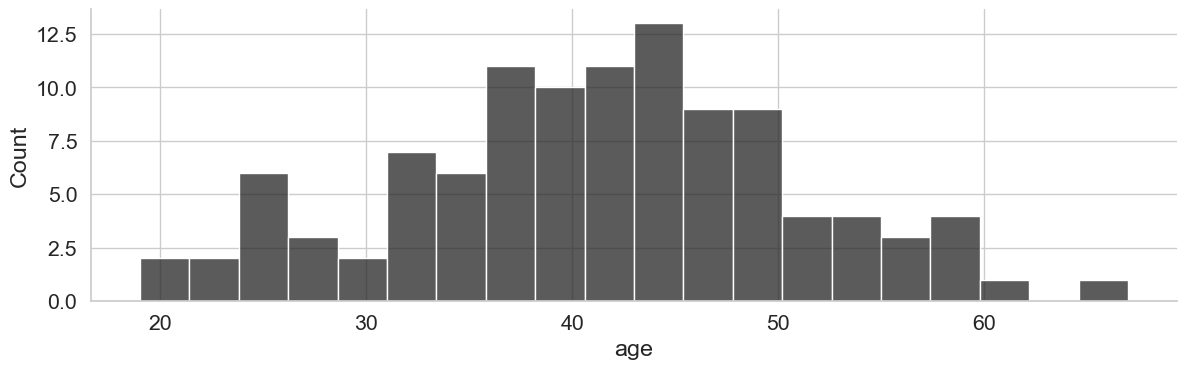
\includegraphics[height=50mm]{./figure/sec4/respondent_dist.png}
%     \caption{被験者の年齢分布}
%     \label{sec4:fig:respondent_dist}
% \end{figure}

% 次に、手法ごとの明瞭性における評価値分布を図~\ref{sec4:fig:int_score_pct}に示す。この図は横軸をモデルのID、縦軸を評価値の割合としてプロットしたものである。また、図~\ref{sec4:fig:int_summary_stats}に手法ごとの明瞭性における評価値平均と95\%信頼区間をプロットしたグラフ、表\ref{sec4:tab:int_summary_stats}にその具体的な値をそれぞれ示す。この図は横軸をモデルのID、縦軸を評価値としてプロットしたものである。どちらの図についても評価値平均が小さい順に左から並べてプロットしている。これより、左から合成音声が並んでおり、(4)分析合成、(5)原音声が合成音声と比較して高い評価を受けている傾向が見て取れる。自然性についても同様に、評価値分布を図~\ref{sec4:fig:nat_score_pct}、評価値平均と95\%信頼区間を図~\ref{sec4:fig:nat_summary_stats}、表\ref{sec4:tab:nat_summary_stats}にそれぞれ示す。自然性についても明瞭性と同様の傾向が見て取れる。原音声の評価値が最も高く、ついで分析合成、合成音声となることは実験として妥当な結果であり、実験は問題なく行われたと判断した。

% \begin{figure}[bt]
%     \centering
%     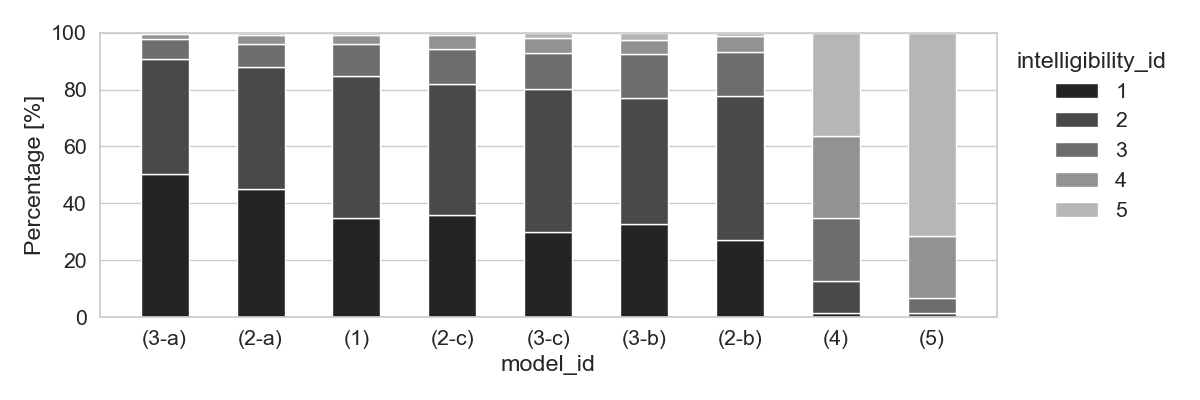
\includegraphics[height=50mm]{./figure/sec4/int_score_pct.png}
%     \caption{手法ごとの明瞭性における評価値分布}
%     \label{sec4:fig:int_score_pct}
% \end{figure}

% \begin{figure}[bt]
%     \centering
%     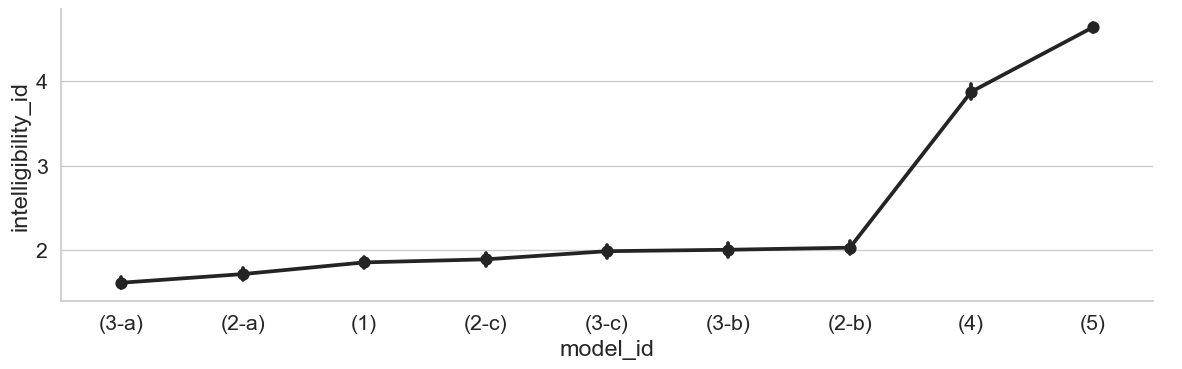
\includegraphics[height=50mm]{./figure/sec4/int_summary_stats.png}
%     \caption{手法ごとの明瞭性における評価値平均と95\%信頼区間(グラフ)}
%     \label{sec4:fig:int_summary_stats}
% \end{figure}

% \begin{table*}[bt]
%     \centering
%     \caption{手法ごとの明瞭性における評価値平均と95\%信頼区間}
%     \label{sec4:tab:int_summary_stats}
%     \begin{center}
%         \renewcommand{\arraystretch}{1.0} % 行の高さ調整
%         \setlength{\tabcolsep}{8pt}      % 列の幅調整
%         \scalebox{0.9}{
%             \begin{tabular}{|l|l|l|r|}
%                 \hline
%                 \multicolumn{1}{|c|}{ID} & \multicolumn{1}{c|}{手法} & \multicolumn{1}{c|}{予測対象} & \multicolumn{1}{c|}{評価値} \\
%                 \hline
%                 (3-a)                    & HuBERTあり                & メル・連続                     & $1.61 \pm 0.03$          \\
%                 (2-a)                    & HuBERTなし                & メル・連続                     & $1.72 \pm 0.04$          \\
%                 (1)                      & ベースライン                  & メル                        & $1.85 \pm 0.04$          \\
%                 (2-c)                    & HuBERTなし                & メル・連続・離散                  & $1.89 \pm 0.04$          \\
%                 (3-c)                    & HuBERTあり                & メル・連続・離散                  & $1.99 \pm 0.04$          \\
%                 (3-b)                    & HuBERTあり                & メル・離散                     & $2.00 \pm 0.04$          \\
%                 (2-b)                    & HuBERTなし                & メル・離散                     & $2.03 \pm 0.04$          \\
%                 (4)                      & 分析合成                    & \multicolumn{1}{c|}{-}    & $3.87 \pm 0.05$          \\
%                 (5)                      & 原音声                     & \multicolumn{1}{c|}{-}    & $4.63 \pm 0.03$          \\
%                 \hline
%             \end{tabular}
%         }
%     \end{center}
% \end{table*}

% \begin{figure}[bt]
%     \centering
%     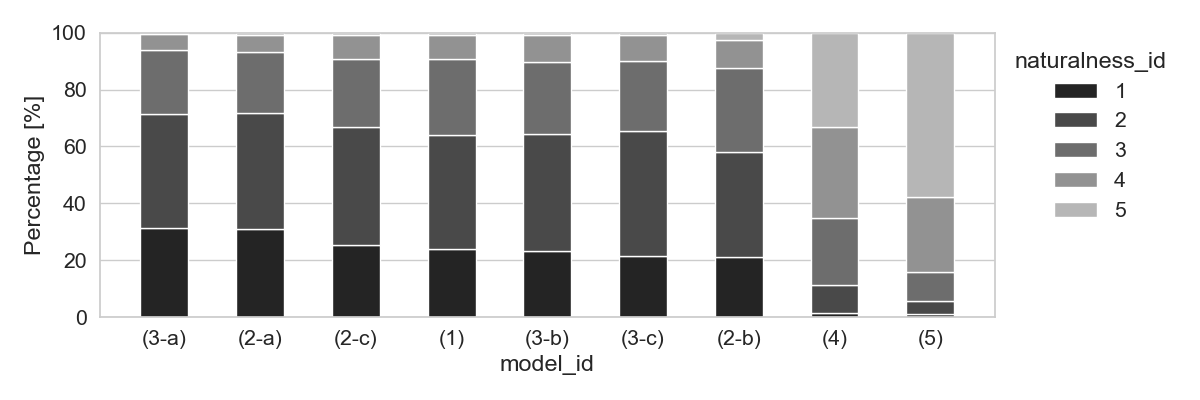
\includegraphics[height=50mm]{./figure/sec4/nat_score_pct.png}
%     \caption{手法ごとの自然性における評価値分布}
%     \label{sec4:fig:nat_score_pct}
% \end{figure}

% \begin{figure}[bt]
%     \centering
%     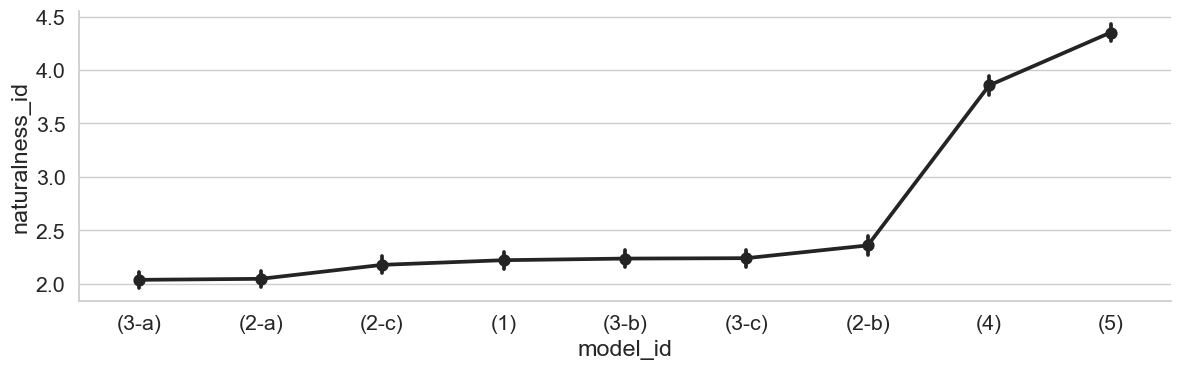
\includegraphics[height=50mm]{./figure/sec4/nat_summary_stats.png}
%     \caption{手法ごとの自然性における評価値平均と95\%信頼区間(グラフ)}
%     \label{sec4:fig:nat_summary_stats}
% \end{figure}

% \begin{table*}[bt]
%     \centering
%     \caption{手法ごとの自然性における評価値平均と95\%信頼区間}
%     \label{sec4:tab:nat_summary_stats}
%     \begin{center}
%         \renewcommand{\arraystretch}{1.0} % 行の高さ調整
%         \setlength{\tabcolsep}{8pt}      % 列の幅調整
%         \scalebox{0.9}{
%             \begin{tabular}{|l|l|l|r|}
%                 \hline
%                 \multicolumn{1}{|c|}{ID} & \multicolumn{1}{c|}{手法} & \multicolumn{1}{c|}{予測対象} & \multicolumn{1}{c|}{評価値} \\
%                 \hline
%                 (3-a)                    & HuBERTあり                & メル・連続                     & $2.04 \pm 0.04$          \\
%                 (2-a)                    & HuBERTなし                & メル・連続                     & $2.05 \pm 0.04$          \\
%                 (2-c)                    & HuBERTなし                & メル・連続・離散                  & $2.18 \pm 0.04$          \\
%                 (1)                      & ベースライン                  & メル                        & $2.22 \pm 0.04$          \\
%                 (3-b)                    & HuBERTあり                & メル・離散                     & $2.24 \pm 0.04$          \\
%                 (3-c)                    & HuBERTあり                & メル・連続・離散                  & $2.24 \pm 0.04$          \\
%                 (2-b)                    & HuBERTなし                & メル・離散                     & $2.36 \pm 0.04$          \\
%                 (4)                      & 分析合成                    & \multicolumn{1}{c|}{-}    & $3.86 \pm 0.05$          \\
%                 (5)                      & 原音声                     & \multicolumn{1}{c|}{-}    & $4.35 \pm 0.04$          \\
%                 \hline
%             \end{tabular}
%         }
%     \end{center}
% \end{table*}

% この評価データを用いて評価値平均に対するt検定を実施することで、手法間の有意差の有無を評価した。手法間で回答者は同じではないため、二群間が等分散であることを仮定しないウェルチのt検定を実施した。また、平均値が大きい手法について、それが統計的に有意な差であるかに興味があるため、有意水準5\%で片側検定を実施した。加えて、手法の組み合わせが多数存在することから、Benjamini-Hochberg法によってp値を補正した。得られたp値をまとめた結果が、表~\ref{sec4:tab:int_ttest}, ~\ref{sec4:tab:nat_ttest}である。この表のi行j列に示す値は、手法i、jの評価平均をそれぞれ$\mu_{i}$、$\mu_{j}$とすると、帰無仮説を「$\mu_{i} = \mu_{j}$」、対立仮説を「$\mu_{i} > \mu_{j}$」とした時のp値である。有意水準5\%で有意差が認められた組み合わせは、下線を引いて示している。

% この結果に対して、以下の三つの観点で考える。
% \begin{enumerate}
%     \item 最も評価の高かった手法は何だったか
%     \item HuBERT導入による効果はあったか
%     \item 予測対象の違いは合成音声の品質に影響を与えたか
% \end{enumerate}

% まず、最も評価の高かった手法は何だったかについて、表~\ref{sec4:tab:int_ttest}を見ると、手法(2-b)、(3-b)、(3-c)がその他の4つの手法に対して有意に評価が高いことが分かる。これより、これら三つの手法はその他の4つの合成音声と比較して、明瞭性が高かったと考えられる。さらに、表~\ref{sec4:tab:nat_ttest}を見ると、手法(2-b)がその他の6つの手法に対して有意に評価が高いことが分かる。これより、評価対象とした合成音声の中で、(2-b)は最も自然性が高かったと考えられる。以上の結果から、今回比較した手法の中で最も評価が高かったのは(2-b)だと考えられ、これはHuBERTなしで音声SSL離散特徴量を予測対象とした先行研究~\cite{choi2023intelligible}の手法である。これは先行研究~\cite{choi2023intelligible}の有効性の指示する結果となり、本研究で新たに提案したHuBERTを導入するアプローチは、この手法を超えることができなかったと言える。

% 次に、HuBERT導入による効果について調べるため、同じ予測対象でHuBERTの有無のみに違いがある、(2-a)と(3-a)、(2-b)と(3-b)、(2-c)と(3-c)の間における有意差の有無に着目する。これら3つのペアのみにおける有意差の有無をまとめた結果を表~\ref{sec4:tab:ttest_hubert}に示す。ここでは有意差のある場合を不等号、ない場合を等号で示している。まず、(2-a)と(3-a)の結果を見ると、明瞭性では(2-a)が有意に高く、自然性では有意差がないことが分かる。次に、(2-b)と(3-b)の結果を見ると、明瞭性では有意差がなく、自然性では(2-b)が有意に高いことが分かる。これらより、HuBERTの導入によって明瞭性あるいは自然性が悪化していると考えられる。しかし、(2-c)と(3-c)の結果を見ると、明瞭性では(3-c)が有意に高く、自然性では有意差がないことが分かる。これは前述した傾向と異なり、HuBERT導入が明瞭性の向上に寄与したと考えられる。従って、本研究で提案したHuBERT導入の有効性は、モデルの予測対象によって異なると考えられる。

% 最後に、予測対象の違いによる変化について調べるため、HuBERTの有無で共通していて予測対象のみに違いがある、(2-a)と(2-b)と(2-c)、(3-a)と(3-b)と(3-c)の間における有意差の有無に着目した。この結果を表~\ref{sec4:tab:ttest_pred}に示す。ここでも有意差のある場合を不等号、ない場合を等号で示している。まず、(2-a)と(2-b)と(2-c)の結果を見ると、明瞭性・自然性どちらにおいても共通して、(2-b)が最も有意に高く、ついで(2-c)、(2-a)が続いて有意に低くなっていることが分かる。これより、HuBERTなしの条件下では予測対象の違いによって明瞭性・自然性ともに有意差が出ており、今回の条件下ではメルスペクトログラムと音声SSL離散特徴量を予測対象とした場合が最も良い評価を得たと言える。次に、(3-a)と(3-b)と(3-c)の結果を見ると、明瞭性・自然性ともに(3-b)と(3-c)の有意差がなくなっていることが分かる。この点がHuBERTなしの場合との違いであり、音声SSL離散特徴量のみを予測対象とする場合と、離散特徴量と連続特徴量の両方を使うアプローチにおける差が小さくなったと考えられる。最後に、メルスペクトログラムと音声SSL連続特徴量を予測対象とした(2-a)、(3-a)はHuBERTの有無によらず有意に評価が低くなっていることが分かる。これより、音声SSLモデルから得られる特徴量を連続値のまま予測対象とするアプローチは、離散化させるアプローチと比較して有効でないと考えられる。連続特徴量はそれを離散化させた特徴量と比較して、より複雑であることが予想される。これを正確に推定しようとするよりも、離散化させてある程度冗長性を省いたものを予測対象とした方が、結果的に合成音声の品質改善につながるのだと考えられる。

% \begin{table*}[bt]
%     \centering
%     \caption{明瞭性の評価値平均に対するt検定の結果}
%     \label{sec4:tab:int_ttest}
%     \begin{center}
%         \renewcommand{\arraystretch}{1.0} % 行の高さ調整
%         \setlength{\tabcolsep}{8pt}      % 列の幅調整
%         \scalebox{0.65}{
%             \begin{tabular}{|l|l|l|l|l|l|l|l|l|l|}
%                 \hline
%                       & \multicolumn{1}{c|}{(4)}    & \multicolumn{1}{c|}{(2-b)}  & \multicolumn{1}{c|}{(3-b)}  & \multicolumn{1}{c|}{(3-c)}  & \multicolumn{1}{c|}{(2-c)}  & \multicolumn{1}{c|}{(1)}    & \multicolumn{1}{c|}{(2-a)}  & \multicolumn{1}{c|}{(3-a)}  \\
%                 \hline
%                 (5)   & \underline{\num{4.52e-40 }} & \underline{\num{9.47e-303}} & \underline{\num{4.67e-280}} & \underline{\num{2.23e-298}} & \underline{\num{1.41e-320}} & \underline{0.00           } & \underline{0.00           } & \underline{0.00           } \\
%                 (4)   & \multicolumn{1}{c|}{-}      & \underline{\num{2.12e-147}} & \underline{\num{4.99e-143}} & \underline{\num{1.22e-149}} & \underline{\num{1.50e-163}} & \underline{\num{3.73e-172}} & \underline{\num{3.92e-188}} & \underline{\num{8.84e-205}} \\
%                 (2-b) & \multicolumn{1}{c|}{-}      & \multicolumn{1}{c|}{-}      & 0.34                        & 0.24                        & \underline{\num{6.06e-03 }} & \underline{\num{5.27e-04 }} & \underline{\num{1.63e-09 }} & \underline{\num{1.32e-16 }} \\
%                 (3-b) & \multicolumn{1}{c|}{-}      & \multicolumn{1}{c|}{-}      & \multicolumn{1}{c|}{-}      & 0.38                        & \underline{0.02           } & \underline{\num{3.92e-03 }} & \underline{\num{1.14e-07 }} & \underline{\num{1.63e-13 }} \\
%                 (3-c) & \multicolumn{1}{c|}{-}      & \multicolumn{1}{c|}{-}      & \multicolumn{1}{c|}{-}      & \multicolumn{1}{c|}{-}      & \underline{0.04           } & \underline{\num{7.19e-03 }} & \underline{\num{2.32e-07 }} & \underline{\num{2.34e-13 }} \\
%                 (2-c) & \multicolumn{1}{c|}{-}      & \multicolumn{1}{c|}{-}      & \multicolumn{1}{c|}{-}      & \multicolumn{1}{c|}{-}      & \multicolumn{1}{c|}{-}      & 0.26                        & \underline{\num{5.27e-04 }} & \underline{\num{2.07e-08 }} \\
%                 (1)   & \multicolumn{1}{c|}{-}      & \multicolumn{1}{c|}{-}      & \multicolumn{1}{c|}{-}      & \multicolumn{1}{c|}{-}      & \multicolumn{1}{c|}{-}      & \multicolumn{1}{c|}{-}      & \underline{\num{3.71e-03 }} & \underline{\num{3.29e-07 }} \\
%                 (2-a) & \multicolumn{1}{c|}{-}      & \multicolumn{1}{c|}{-}      & \multicolumn{1}{c|}{-}      & \multicolumn{1}{c|}{-}      & \multicolumn{1}{c|}{-}      & \multicolumn{1}{c|}{-}      & \multicolumn{1}{c|}{-}      & \underline{0.02           } \\
%                 \hline
%             \end{tabular}
%         }
%     \end{center}
% \end{table*}

% \begin{table*}[bt]
%     \centering
%     \caption{自然性の評価値平均に対するt検定の結果}
%     \label{sec4:tab:nat_ttest}
%     \begin{center}
%         \renewcommand{\arraystretch}{1.0} % 行の高さ調整
%         \setlength{\tabcolsep}{8pt}      % 列の幅調整
%         \scalebox{0.65}{
%             \begin{tabular}{|l|l|l|l|l|l|l|l|l|l|}
%                 \hline
%                       & \multicolumn{1}{c|}{(4)}    & \multicolumn{1}{c|}{(2-b)}  & \multicolumn{1}{c|}{(3-c)}  & \multicolumn{1}{c|}{(3-b)}  & \multicolumn{1}{c|}{(1)}    & \multicolumn{1}{c|}{(2-c)}  & \multicolumn{1}{c|}{(2-a)}  & \multicolumn{1}{c|}{(3-a)}  \\
%                 \hline
%                 (5)   & \underline{\num{7.94e-16 }} & \underline{\num{1.21e-168}} & \underline{\num{1.24e-193}} & \underline{\num{2.03e-191}} & \underline{\num{5.14e-194}} & \underline{\num{2.23e-200}} & \underline{\num{3.49e-219}} & \underline{\num{1.02e-221}} \\
%                 (4)   & \multicolumn{1}{c|}{-}      & \underline{\num{6.24e-101}} & \underline{\num{3.64e-120}} & \underline{\num{4.86e-119}} & \underline{\num{3.23e-121}} & \underline{\num{8.06e-127}} & \underline{\num{1.18e-143}} & \underline{\num{1.03e-145}} \\
%                 (2-b) & \multicolumn{1}{c|}{-}      & \multicolumn{1}{c|}{-}      & \underline{0.03           } & \underline{0.03           } & \underline{0.01           } & \underline{\num{1.71e-03 }} & \underline{\num{1.41e-07 }} & \underline{\num{5.32e-08 }} \\
%                 (3-c) & \multicolumn{1}{c|}{-}      & \multicolumn{1}{c|}{-}      & \multicolumn{1}{c|}{-}      & 0.47                        & 0.40                        & 0.16                        & \underline{\num{5.79e-04 }} & \underline{\num{3.18e-04 }} \\
%                 (3-b) & \multicolumn{1}{c|}{-}      & \multicolumn{1}{c|}{-}      & \multicolumn{1}{c|}{-}      & \multicolumn{1}{c|}{-}      & 0.42                        & 0.18                        & \underline{\num{7.96e-04 }} & \underline{\num{4.47e-04 }} \\
%                 (1)   & \multicolumn{1}{c|}{-}      & \multicolumn{1}{c|}{-}      & \multicolumn{1}{c|}{-}      & \multicolumn{1}{c|}{-}      & \multicolumn{1}{c|}{-}      & 0.25                        & \underline{\num{1.71e-03 }} & \underline{\num{9.69e-04 }} \\
%                 (2-c) & \multicolumn{1}{c|}{-}      & \multicolumn{1}{c|}{-}      & \multicolumn{1}{c|}{-}      & \multicolumn{1}{c|}{-}      & \multicolumn{1}{c|}{-}      & \multicolumn{1}{c|}{-}      & \underline{0.01           } & \underline{\num{9.27e-03 }} \\
%                 (2-a) & \multicolumn{1}{c|}{-}      & \multicolumn{1}{c|}{-}      & \multicolumn{1}{c|}{-}      & \multicolumn{1}{c|}{-}      & \multicolumn{1}{c|}{-}      & \multicolumn{1}{c|}{-}      & \multicolumn{1}{c|}{-}      & 0.44                        \\
%                 \hline
%             \end{tabular}
%         }
%     \end{center}
% \end{table*}

% \begin{table*}[bt]
%     \centering
%     \caption{HuBERTの有無に対する比較}
%     \label{sec4:tab:ttest_hubert}
%     \begin{center}
%         \renewcommand{\arraystretch}{0.9} % 行の高さ調整
%         \setlength{\tabcolsep}{8pt}      % 列の幅調整
%         \scalebox{1.0}{
%             \begin{tabular}{|l|c|c|}
%                 \hline
%                             & \multicolumn{1}{c|}{明瞭性} & \multicolumn{1}{c|}{自然性} \\
%                 \hline
%                 (2-a)、(3-a) & (2-a) $>$ (3-a)          & (2-a) = (3-a)            \\
%                 (2-b)、(3-b) & (2-b) = (3-b)            & (2-b) $>$ (3-b)          \\
%                 (2-c)、(3-c) & (2-c) $<$ (3-c)          & (2-c) = (3-c)            \\
%                 \hline
%             \end{tabular}
%         }
%     \end{center}
% \end{table*}

% \begin{table*}[bt]
%     \centering
%     \caption{予測対象による比較}
%     \label{sec4:tab:ttest_pred}
%     \begin{center}
%         \renewcommand{\arraystretch}{0.9} % 行の高さ調整
%         \setlength{\tabcolsep}{8pt}      % 列の幅調整
%         \scalebox{1.0}{
%             \begin{tabular}{|l|c|c|}
%                 \hline
%                                   & \multicolumn{1}{c|}{明瞭性}  & \multicolumn{1}{c|}{自然性}  \\
%                 \hline
%                 (2-a)、(2-b)、(2-c) & (2-b) $>$ (2-c) $>$ (2-a) & (2-b) $>$ (2-c) $>$ (2-a) \\
%                 (3-a)、(3-b)、(3-c) & (3-b) = (3-c) $>$ (3-a)   & (3-b) = (3-c) $>$ (3-a)   \\
%                 \hline
%             \end{tabular}
%         }
%     \end{center}
% \end{table*}

% \clearpage

% \subsection{まとめ}
% 本章では、音声SSLモデルであるHuBERTを利用した動画音声合成モデルを提案し、既存手法との比較を行った。

% 客観評価では、HuBERTを利用してメルスペクトログラムと音声SSL連続特徴量、離散特徴量を予測対象とした手法が、PESQ、STOI、ESTOIにおいて最も高い評価を得た。しかし、WERにおいてはHuBERTなしでメルスペクトログラムと音声SSL離散特徴量を予測対象とした手法が最も低く、提案手法に課題が残った。主観評価では、客観評価においてWERが最も低かった、HuBERTなしでメルスペクトログラムと音声SSL離散特徴量を予測対象とした手法が最も高い評価を得た。本研究で提案した手法もそれに次ぐような評価ではあったが、特に自然性については有意に低く、既存手法に対する提案手法の有効性は示されなかった。また、HuBERTの導入による効果の良し悪しはモデルの予測対象によって異なること、予測対象として音声SSL連続特徴量を直接推定するアプローチでは有効ではなさそうだということがわかった。

% 今後の研究では、提案手法の更なる改善に取り組む必要があると考える。本章では、改めて既存手法の有効性が示されたものの、得られる合成音声の品質は未だ低い。実際、主観評価実験の結果から、分析合成や原音声と合成音声の間の差は顕著であることが分かる。代用音声として利用する上ではより自然な音声であることが望ましく、既存手法を超える品質を達成する、新たな手法の検討が今後も必要だと考える。また、提案手法について課題が残る結果となったが、学習方法や予測方法に改善の余地があるのではないかと考えている。例えば、今回のHuBERTの学習ではすべての重みを更新するようFineTuningしたが、少量の音声データでチューニングした結果として、事前学習によって得た知識を忘却してしまう破滅的忘却に陥っていた可能性があり、これを防止するような学習を施すことが有効な可能性がある。また、HuBERTの事前学習ではマスク部分を推定するが、この際には正しいフレームを参照可能である。しかし、今回のFineTuningでは初めから推定結果のみを入力としていたため正しいフレームが存在せず、この条件のギャップが転移学習を困難にしていた可能性がある。これに対して、初めは合成音声にあえて原音声を混入させたものを入力として学習し、それを徐々に完全な合成音声に近づけるような方法ならば、転移学習をより効果的に行える可能性がある。最後に、今回はHuBERTのみから音声SSL特徴量を推定するような形でネットワークを提案したが、AVHuBERTから同時に予測するような枠組みとしても良いと考えている。先行研究が有効であったことも考慮すると、AVHuBERTから予測した結果とHuBERTから予測した結果を両方利用するようなアプローチも、改善の可能性があると考える。

% \clearpage

% \section{音声SSLモデルを活用した動画音声合成の再検討}
% \subsection{客観評価指標の見直し}
% これまでに用いてきた四つの客観評価指標は、動画音声合成において一般的に用いられていることから採用していた。しかし、音声合成において本質的に重要なのは、人が実際に聞いた上で良いと思うか、すなわち主観評価の良し悪しであると考える。そこで、主観評価実験における評価平均値と、客観評価指標の間で計算した相関係数を表に示す。
% これより、明瞭性においてはESTOIおよびWERの相関係数の絶対値が0.9と同程度に高く、PESQやSTOIはこれらと比較して相関係数の絶対値が小さい。
% また、自然性においてはWERの相関係数の絶対値が0.911と再び高いが、PESQ、STOI、ESTOIはこれと比較して相関係数の絶対値が小さい。
% 以上の結果から、従来一般的に用いられてきた客観評価指標の中でPESQ、STOI、ESTOIは主観評価との相関が比較的弱く、主観評価実験に向けたモデルのチューニングを行っていく上では、WERが最も信頼できる指標であると判断する。
% 加えて、表では近年提案されたMOS値の自動評価モデルである、UTMOSによって得られた評価値についての相関係数も掲載している。これを見ると、特に明瞭性においてその相関係数は0.986と高く、自然性との相関係数も0.882となっており、WERと同程度の高い値を示している。
% これより、本セクション以降ではこれまで用いてきた客観評価指標を改め、主観評価との相関が高いWERとUTMOSによって合成音声の客観評価を行うこととする。

% \begin{table*}[b]
%     \centering
%     \caption{予測対象による比較}
%     \label{sec5:tab:obj_comp}
%     \begin{center}
%         \renewcommand{\arraystretch}{0.9} % 行の高さ調整
%         \setlength{\tabcolsep}{8pt}      % 列の幅調整
%         \scalebox{1.0}{
%             \begin{tabular}{|l|c|c|}
%                 \hline
%                       & \multicolumn{1}{c|}{明瞭性} & \multicolumn{1}{c|}{自然性} \\
%                 \hline
%                 PESQ  & 0.671                    & 0.523                    \\
%                 STOI  & 0.690                    & 0.676                    \\
%                 ESTOI & 0.900                    & 0.749                    \\
%                 WER   & -0.900                   & -0.911                   \\
%                 UTMOS & 0.986                    & 0.882                    \\
%                 \hline
%             \end{tabular}
%         }
%     \end{center}
% \end{table*}

% \clearpage

\section{結論}

\clearpage

\section*{謝辞}
\addcontentsline{toc}{section}{謝辞}

\clearpage

\bibliographystyle{junsrt}
\addcontentsline{toc}{section}{参考文献}
\bibliography{library}

\end{document}